\ifx\master\undefined% AUTOCOMPILE
% Allows for individual chapters to be compiled.

% Usage:
% \ifx\master\undefined% AUTOCOMPILE
% Allows for individual chapters to be compiled.

% Usage:
% \ifx\master\undefined% AUTOCOMPILE
% Allows for individual chapters to be compiled.

% Usage:
% \ifx\master\undefined\input{../settings/autocompile}\fi
% (place at start and end of chapter file)

\ifx\noprelim\undefined
    % first time included
    % input preamble files
    \input{../settings/phdsetup}

    \begin{document}
    \def\noprelim{}
\else
    % already included once
    % input post files

    \singlespacing
    \bibliographystyle{../bibliography/expanded}
    \bibliography{../bibliography/references}

    \end{document}
\fi\fi
% (place at start and end of chapter file)

\ifx\noprelim\undefined
    % first time included
    % input preamble files
    % [ USER VARIABLES ]

\def\PHDTITLE {Extensions of the Theory of Computational Mechanics}
\def\PHDAUTHOR{Evan Klose Friis}
\def\PHDSCHOOL{University of California, Davis}

\def\PHDMONTH {June}
\def\PHDYEAR  {2011}
\def\PHDDEPT {Physics}

\def\BSSCHOOL {University of California at San Diego}
\def\BSYEAR   {2005}

\def\PHDCOMMITTEEA{Professor John Conway}
\def\PHDCOMMITTEEB{Professor Robin Erbacher}
\def\PHDCOMMITTEEC{Professor Mani Tripathi}

% [ GLOBAL SETUP ]

\documentclass[letterpaper,oneside,11pt]{report}

\usepackage{calc}
\usepackage{breakcites}
\usepackage[newcommands]{ragged2e}

\usepackage[pdftex]{graphicx}
\usepackage{epstopdf}

%\usepackage{tikz}
%\usetikzlibrary{positioning} % [right=of ...]
%\usetikzlibrary{fit} % [fit= ...]

%\pgfdeclarelayer{background layer}
%\pgfdeclarelayer{foreground layer}
%\pgfsetlayers{background layer,main,foreground layer}

%\newenvironment{wrap}{\noindent\begin{minipage}[t]{\linewidth}\vspace{-0.5\normalbaselineskip}\centering}{\vspace{0.5\normalbaselineskip}\end{minipage}}

%% [Venn diagram environment]
%\newenvironment{venn2}
%{\begin{tikzpicture} [every pin/.style={text=black, text opacity=1.0, pin distance=0.5cm, pin edge={black!60, semithick}},
%% define a new style 'venn'
%venn/.style={circle, draw=black!60, semithick, minimum size = 4cm}]
%
%% create circle and give it external (pin) label
%\node[venn] (X) at (-1,0) [pin={150:$H[X]$}] {};
%\node[venn] (Y) at (1,0) [pin={30:$H[Y]$}] {};
%
%% place labels of the atoms by hand
%\node at (-1.9,0) {$H[X|Y]$};
%\node at (1.9,0) {$H[Y|X]$};
%\node at (0,0) {$I[X;Y]$};}
%{\end{tikzpicture}}

%\newcommand{\wrapmath}[1]{\begin{wrap}\begin{tikzpicture}[every node/.style={inner ysep=0ex, inner xsep=0em}]\node[] {$\displaystyle\begin{aligned} #1\end{aligned}$};\end{tikzpicture}\end{wrap}}

\renewenvironment{abstract}{\chapter*{Abstract}}{}
\renewcommand{\bibname}{Bibliography}
\renewcommand{\contentsname}{Table of Contents}

\makeatletter
\renewcommand{\@biblabel}[1]{\textsc{#1}}
\makeatother

% [ FONT SETTINGS ]

\usepackage[tbtags, intlimits, namelimits]{amsmath}
\usepackage[adobe-utopia]{mathdesign}

\DeclareSymbolFont{pazomath}{OMS}{zplm}{m}{n}
\DeclareSymbolFontAlphabet{\mathcal}{pazomath}
\SetMathAlphabet\mathcal{bold}{OMS}{zplm}{b}{n}

\SetSymbolFont{largesymbols}{normal}{OMX}{zplm}{m}{n}
\SetSymbolFont{largesymbols}{bold}{OMX}{zplm}{m}{n}
\SetSymbolFont{symbols}{normal}{OMS}{zplm}{m}{n}
\SetSymbolFont{symbols}{bold}{OMS}{zplm}{b}{n}

\renewcommand{\sfdefault}{phv}
\renewcommand{\ttdefault}{fvm}

\widowpenalty 8000
\clubpenalty  8000

% [ PAGE LAYOUT ]
\usepackage{geometry}
\geometry{lmargin = 1.5in}
\geometry{rmargin = 1.0in}
\geometry{tmargin = 1.0in}
\geometry{bmargin = 1.0in}

% [ PDF SETTINGS ]

\usepackage[final]{hyperref}
\hypersetup{breaklinks  = true}
\hypersetup{colorlinks  = true}
\hypersetup{linktocpage = false}
\hypersetup{linkcolor   = blue}
\hypersetup{citecolor   = green}
\hypersetup{urlcolor    = black}
\hypersetup{plainpages  = false}
\hypersetup{pageanchor  = true}
\hypersetup{pdfauthor   = {\PHDAUTHOR}}
\hypersetup{pdftitle    = {\PHDTITLE}}
\hypersetup{pdfsubject  = {Dissertation, \PHDSCHOOL}}
\urlstyle{same}

% [ LETTER SPACING ]

\usepackage[final]{microtype}
\microtypesetup{protrusion=compatibility}
\microtypesetup{expansion=false}

\newcommand{\upper}[1]{\MakeUppercase{#1}}
\let\lsscshape\scshape

\ifcase\pdfoutput\else\microtypesetup{letterspace=15}
\renewcommand{\scshape}{\lsscshape\lsstyle}
\renewcommand{\upper}[1]{\textls[50]{\MakeUppercase{#1}}}\fi

% [ LINE SPACING ]

\usepackage[doublespacing]{setspace}
\renewcommand{\displayskipstretch}{0.0}

\setlength{\parskip   }{0em}
\setlength{\parindent }{2em}

% [ TABLE FORMATTING ]

\usepackage{booktabs}
\setlength{\heavyrulewidth}{1.5\arrayrulewidth}
\setlength{\lightrulewidth}{1.0\arrayrulewidth}
\setlength{\doublerulesep }{2.0\arrayrulewidth}

% [ SECTION FORMATTING ]

\usepackage[largestsep,nobottomtitles*]{titlesec}
\renewcommand{\bottomtitlespace}{0.75in}

\titleformat{\chapter}[display]{\bfseries\huge\singlespacing}{\filleft\textsc{\LARGE \chaptertitlename\ \thechapter}}{-0.2ex}{\titlerule[3pt]\vspace{0.2ex}}[]

\titleformat{\section}{\LARGE}{\S\thesection\hspace{0.5em}}{0ex}{}
\titleformat{\subsection}{\Large}{\S\thesubsection\hspace{0.5em}}{0ex}{}
\titleformat{\subsubsection}{\large}{\thesubsubsection\hspace{0.5em}}{0ex}{}

\titlespacing*{\chapter}{0em}{6ex}{4ex plus 2ex minus 0ex}
\titlespacing*{\section}{0em}{2ex plus 3ex minus 1ex}{0.5ex plus 0.5ex minus 0.5ex}
\titlespacing*{\subsection}{0ex}{2ex plus 3ex minus 1ex}{0ex}
\titlespacing*{\subsubsection}{0ex}{2ex plus 0ex minus 1ex}{0ex}

% [ HEADER SETTINGS ]

\usepackage{fancyhdr}

\setlength{\headheight}{\normalbaselineskip}
\setlength{\footskip  }{0.5in}
\setlength{\headsep   }{0.5in-\headheight}

\fancyheadoffset[R]{0.5in}
\renewcommand{\headrulewidth}{0pt}
\renewcommand{\footrulewidth}{0pt}

\newcommand{\pagebox}{\parbox[r][\headheight][t]{0.5in}{\hspace\fill\thepage}}

\newcommand{\prelimheaders}{\ifx\prelim\undefined\renewcommand{\thepage}{\textit{\roman{page}}}\fancypagestyle{plain}{\fancyhf{}\fancyfoot[L]{\makebox[\textwidth-0.5in]{\thepage}}}\pagestyle{plain}\def\prelim{}\fi}

\newcommand{\normalheaders}{\renewcommand{\thepage}{\arabic{page}}\fancypagestyle{plain}{\fancyhf{}\fancyhead[R]{\pagebox}}\pagestyle{plain}}

\normalheaders{}

% [ CUSTOM COMMANDS ]

\newcommand{\signaturebox}[1]{\multicolumn{1}{p{4in}}{\vspace{3ex}}\\\midrule #1\\}

%\input{../includes/cmechabbrev}

% [some math stuff - maybe stick in sep file]
\usepackage{amsthm}
\usepackage{amscd}
\theoremstyle{plain}    \newtheorem{Lem}{Lemma}
\theoremstyle{plain}    \newtheorem*{ProLem}{Proof}
\theoremstyle{plain} 	\newtheorem{Cor}{Corollary}
\theoremstyle{plain} 	\newtheorem*{ProCor}{Proof}
\theoremstyle{plain} 	\newtheorem{The}{Theorem}
\theoremstyle{plain} 	\newtheorem*{ProThe}{Proof}
\theoremstyle{plain} 	\newtheorem{Prop}{Proposition}
\theoremstyle{plain} 	\newtheorem*{ProProp}{Proof}
\theoremstyle{plain} 	\newtheorem*{Conj}{Conjecture}
\theoremstyle{plain}	\newtheorem*{Rem}{Remark}
\theoremstyle{plain}	\newtheorem*{Def}{Definition} 
\theoremstyle{plain}	\newtheorem*{Not}{Notation}

% [uniform figure scaling - maybe this is not a good idea]
\def\figscale{.7}
\def\lscale{1.0}

% [FIX ME! - red makes it easier to spot]
\newcommand{\FIX}[1]{\textbf{\textcolor{red}{#1}}}


    \begin{document}
    \def\noprelim{}
\else
    % already included once
    % input post files

    \singlespacing
    \bibliographystyle{../bibliography/expanded}
    \bibliography{../bibliography/references}

    \end{document}
\fi\fi
% (place at start and end of chapter file)

\ifx\noprelim\undefined
    % first time included
    % input preamble files
    % [ USER VARIABLES ]

\def\PHDTITLE {Extensions of the Theory of Computational Mechanics}
\def\PHDAUTHOR{Evan Klose Friis}
\def\PHDSCHOOL{University of California, Davis}

\def\PHDMONTH {June}
\def\PHDYEAR  {2011}
\def\PHDDEPT {Physics}

\def\BSSCHOOL {University of California at San Diego}
\def\BSYEAR   {2005}

\def\PHDCOMMITTEEA{Professor John Conway}
\def\PHDCOMMITTEEB{Professor Robin Erbacher}
\def\PHDCOMMITTEEC{Professor Mani Tripathi}

% [ GLOBAL SETUP ]

\documentclass[letterpaper,oneside,11pt]{report}

\usepackage{calc}
\usepackage{breakcites}
\usepackage[newcommands]{ragged2e}

\usepackage[pdftex]{graphicx}
\usepackage{epstopdf}

%\usepackage{tikz}
%\usetikzlibrary{positioning} % [right=of ...]
%\usetikzlibrary{fit} % [fit= ...]

%\pgfdeclarelayer{background layer}
%\pgfdeclarelayer{foreground layer}
%\pgfsetlayers{background layer,main,foreground layer}

%\newenvironment{wrap}{\noindent\begin{minipage}[t]{\linewidth}\vspace{-0.5\normalbaselineskip}\centering}{\vspace{0.5\normalbaselineskip}\end{minipage}}

%% [Venn diagram environment]
%\newenvironment{venn2}
%{\begin{tikzpicture} [every pin/.style={text=black, text opacity=1.0, pin distance=0.5cm, pin edge={black!60, semithick}},
%% define a new style 'venn'
%venn/.style={circle, draw=black!60, semithick, minimum size = 4cm}]
%
%% create circle and give it external (pin) label
%\node[venn] (X) at (-1,0) [pin={150:$H[X]$}] {};
%\node[venn] (Y) at (1,0) [pin={30:$H[Y]$}] {};
%
%% place labels of the atoms by hand
%\node at (-1.9,0) {$H[X|Y]$};
%\node at (1.9,0) {$H[Y|X]$};
%\node at (0,0) {$I[X;Y]$};}
%{\end{tikzpicture}}

%\newcommand{\wrapmath}[1]{\begin{wrap}\begin{tikzpicture}[every node/.style={inner ysep=0ex, inner xsep=0em}]\node[] {$\displaystyle\begin{aligned} #1\end{aligned}$};\end{tikzpicture}\end{wrap}}

\renewenvironment{abstract}{\chapter*{Abstract}}{}
\renewcommand{\bibname}{Bibliography}
\renewcommand{\contentsname}{Table of Contents}

\makeatletter
\renewcommand{\@biblabel}[1]{\textsc{#1}}
\makeatother

% [ FONT SETTINGS ]

\usepackage[tbtags, intlimits, namelimits]{amsmath}
\usepackage[adobe-utopia]{mathdesign}

\DeclareSymbolFont{pazomath}{OMS}{zplm}{m}{n}
\DeclareSymbolFontAlphabet{\mathcal}{pazomath}
\SetMathAlphabet\mathcal{bold}{OMS}{zplm}{b}{n}

\SetSymbolFont{largesymbols}{normal}{OMX}{zplm}{m}{n}
\SetSymbolFont{largesymbols}{bold}{OMX}{zplm}{m}{n}
\SetSymbolFont{symbols}{normal}{OMS}{zplm}{m}{n}
\SetSymbolFont{symbols}{bold}{OMS}{zplm}{b}{n}

\renewcommand{\sfdefault}{phv}
\renewcommand{\ttdefault}{fvm}

\widowpenalty 8000
\clubpenalty  8000

% [ PAGE LAYOUT ]
\usepackage{geometry}
\geometry{lmargin = 1.5in}
\geometry{rmargin = 1.0in}
\geometry{tmargin = 1.0in}
\geometry{bmargin = 1.0in}

% [ PDF SETTINGS ]

\usepackage[final]{hyperref}
\hypersetup{breaklinks  = true}
\hypersetup{colorlinks  = true}
\hypersetup{linktocpage = false}
\hypersetup{linkcolor   = blue}
\hypersetup{citecolor   = green}
\hypersetup{urlcolor    = black}
\hypersetup{plainpages  = false}
\hypersetup{pageanchor  = true}
\hypersetup{pdfauthor   = {\PHDAUTHOR}}
\hypersetup{pdftitle    = {\PHDTITLE}}
\hypersetup{pdfsubject  = {Dissertation, \PHDSCHOOL}}
\urlstyle{same}

% [ LETTER SPACING ]

\usepackage[final]{microtype}
\microtypesetup{protrusion=compatibility}
\microtypesetup{expansion=false}

\newcommand{\upper}[1]{\MakeUppercase{#1}}
\let\lsscshape\scshape

\ifcase\pdfoutput\else\microtypesetup{letterspace=15}
\renewcommand{\scshape}{\lsscshape\lsstyle}
\renewcommand{\upper}[1]{\textls[50]{\MakeUppercase{#1}}}\fi

% [ LINE SPACING ]

\usepackage[doublespacing]{setspace}
\renewcommand{\displayskipstretch}{0.0}

\setlength{\parskip   }{0em}
\setlength{\parindent }{2em}

% [ TABLE FORMATTING ]

\usepackage{booktabs}
\setlength{\heavyrulewidth}{1.5\arrayrulewidth}
\setlength{\lightrulewidth}{1.0\arrayrulewidth}
\setlength{\doublerulesep }{2.0\arrayrulewidth}

% [ SECTION FORMATTING ]

\usepackage[largestsep,nobottomtitles*]{titlesec}
\renewcommand{\bottomtitlespace}{0.75in}

\titleformat{\chapter}[display]{\bfseries\huge\singlespacing}{\filleft\textsc{\LARGE \chaptertitlename\ \thechapter}}{-0.2ex}{\titlerule[3pt]\vspace{0.2ex}}[]

\titleformat{\section}{\LARGE}{\S\thesection\hspace{0.5em}}{0ex}{}
\titleformat{\subsection}{\Large}{\S\thesubsection\hspace{0.5em}}{0ex}{}
\titleformat{\subsubsection}{\large}{\thesubsubsection\hspace{0.5em}}{0ex}{}

\titlespacing*{\chapter}{0em}{6ex}{4ex plus 2ex minus 0ex}
\titlespacing*{\section}{0em}{2ex plus 3ex minus 1ex}{0.5ex plus 0.5ex minus 0.5ex}
\titlespacing*{\subsection}{0ex}{2ex plus 3ex minus 1ex}{0ex}
\titlespacing*{\subsubsection}{0ex}{2ex plus 0ex minus 1ex}{0ex}

% [ HEADER SETTINGS ]

\usepackage{fancyhdr}

\setlength{\headheight}{\normalbaselineskip}
\setlength{\footskip  }{0.5in}
\setlength{\headsep   }{0.5in-\headheight}

\fancyheadoffset[R]{0.5in}
\renewcommand{\headrulewidth}{0pt}
\renewcommand{\footrulewidth}{0pt}

\newcommand{\pagebox}{\parbox[r][\headheight][t]{0.5in}{\hspace\fill\thepage}}

\newcommand{\prelimheaders}{\ifx\prelim\undefined\renewcommand{\thepage}{\textit{\roman{page}}}\fancypagestyle{plain}{\fancyhf{}\fancyfoot[L]{\makebox[\textwidth-0.5in]{\thepage}}}\pagestyle{plain}\def\prelim{}\fi}

\newcommand{\normalheaders}{\renewcommand{\thepage}{\arabic{page}}\fancypagestyle{plain}{\fancyhf{}\fancyhead[R]{\pagebox}}\pagestyle{plain}}

\normalheaders{}

% [ CUSTOM COMMANDS ]

\newcommand{\signaturebox}[1]{\multicolumn{1}{p{4in}}{\vspace{3ex}}\\\midrule #1\\}

%%%% macros fro standard references
%\eqref provided by amsmath
\newcommand{\figref}[1]{Fig.~\ref{#1}}
\newcommand{\tableref}[1]{Table~\ref{#1}}
\newcommand{\refcite}[1]{Ref.~\cite{#1}}

% Abbreviations from CMPPSS:

\newcommand{\eM}     {\mbox{$\epsilon$-machine}}
\newcommand{\eMs}    {\mbox{$\epsilon$-machines}}
\newcommand{\EM}     {\mbox{$\epsilon$-Machine}}
\newcommand{\EMs}    {\mbox{$\epsilon$-Machines}}
\newcommand{\eT}     {\mbox{$\epsilon$-transducer}}
\newcommand{\eTs}    {\mbox{$\epsilon$-transducers}}
\newcommand{\ET}     {\mbox{$\epsilon$-Transducer}}
\newcommand{\ETs}    {\mbox{$\epsilon$-Transducers}}

% Processes and sequences

\newcommand{\Process}{\mathcal{P}}

\newcommand{\ProbMach}{\Prob_{\mathrm{M}}}
\newcommand{\Lmax}   { {L_{\mathrm{max}}}}
\newcommand{\MeasAlphabet}	{\mathcal{A}}
% Original
%\newcommand{\MeasSymbol}   { {S} }
%\newcommand{\meassymbol}   { {s} }
% New symbol
\newcommand{\MeasSymbol}   { {X} }
\newcommand{\meassymbol}   { {x} }
\newcommand{\BiInfinity}	{ \overleftrightarrow {\MeasSymbol} }
\newcommand{\biinfinity}	{ \overleftrightarrow {\meassymbol} }
\newcommand{\Past}	{ \overleftarrow {\MeasSymbol} }
\newcommand{\past}	{ {\overleftarrow {\meassymbol}} }
\newcommand{\pastprime}	{ {\past}^{\prime}}
\newcommand{\Future}	{ \overrightarrow{\MeasSymbol} }
\newcommand{\future}	{ \overrightarrow{\meassymbol} }
\newcommand{\futureprime}	{ {\future}^{\prime}}
\newcommand{\PastPrime}	{ {\Past}^{\prime}}
\newcommand{\FuturePrime}	{ {\overrightarrow{\meassymbol}}^\prime }
\newcommand{\PastDblPrime}	{ {\overleftarrow{\meassymbol}}^{\prime\prime} }
\newcommand{\FutureDblPrime}	{ {\overrightarrow{\meassymbol}}^{\prime\prime} }
\newcommand{\pastL}	{ {\overleftarrow {\meassymbol}}{}^L }
\newcommand{\PastL}	{ {\overleftarrow {\MeasSymbol}}{}^L }
\newcommand{\PastLt}	{ {\overleftarrow {\MeasSymbol}}_t^L }
\newcommand{\PastLLessOne}	{ {\overleftarrow {\MeasSymbol}}^{L-1} }
\newcommand{\futureL}	{ {\overrightarrow{\meassymbol}}{}^L }
\newcommand{\FutureL}	{ {\overrightarrow{\MeasSymbol}}{}^L }
\newcommand{\FutureLt}	{ {\overrightarrow{\MeasSymbol}}_t^L }
\newcommand{\FutureLLessOne}	{ {\overrightarrow{\MeasSymbol}}^{L-1} }
\newcommand{\pastLprime}	{ {\overleftarrow {\meassymbol}}^{L^\prime} }
\newcommand{\futureLprime}	{ {\overrightarrow{\meassymbol}}^{L^\prime} }
\newcommand{\AllPasts}	{ { \overleftarrow {\rm {\bf \MeasSymbol}} } }
\newcommand{\AllFutures}	{ \overrightarrow {\rm {\bf \MeasSymbol}} }
\newcommand{\FutureSet}	{ \overrightarrow{\bf \MeasSymbol}}

% Causal states and epsilon-machines
\newcommand{\CausalState}	{ \mathcal{S} }
\newcommand{\CausalStatePrime}	{ {\CausalState}^{\prime}}
\newcommand{\causalstate}	{ \sigma }
\newcommand{\CausalStateSet}	{ \boldsymbol{\CausalState} }
\newcommand{\AlternateState}	{ \mathcal{R} }
\newcommand{\AlternateStatePrime}	{ {\cal R}^{\prime} }
\newcommand{\alternatestate}	{ \rho }
\newcommand{\alternatestateprime}	{ {\rho^{\prime}} }
\newcommand{\AlternateStateSet}	{ \boldsymbol{\AlternateState} }
\newcommand{\PrescientState}	{ \widehat{\AlternateState} }
\newcommand{\prescientstate}	{ \widehat{\alternatestate} }
\newcommand{\PrescientStateSet}	{ \boldsymbol{\PrescientState}}
\newcommand{\CausalEquivalence}	{ {\sim}_{\epsilon} }
\newcommand{\CausalEquivalenceNot}	{ {\not \sim}_{\epsilon}}

\newcommand{\NonCausalEquivalence}	{ {\sim}_{\eta} }
\newcommand{\NextObservable}	{ {\overrightarrow {\MeasSymbol}}^1 }
\newcommand{\LastObservable}	{ {\overleftarrow {\MeasSymbol}}^1 }
%\newcommand{\Prob}		{ {\rm P}}
\newcommand{\Prob}      {\Pr} % use standard command
\newcommand{\ProbAnd}	{ {,\;} }
\newcommand{\LLimit}	{ {L \rightarrow \infty}}
\newcommand{\Cmu}		{C_\mu}
\newcommand{\hmu}		{h_\mu}
\newcommand{\EE}		{{\bf E}}
\newcommand{\Measurable}{{\bf \mu}}

% Process Crypticity
\newcommand{\PC}		{\chi}
\newcommand{\FuturePC}		{\PC^+}
\newcommand{\PastPC}		{\PC^-}
% Causal Irreversibility
\newcommand{\CI}		{\Xi}
\newcommand{\ReverseMap}	{r}
\newcommand{\ForwardMap}	{f}

% Abbreviations from IB:
% None that aren't already in CMPPSS

% Abbreviations from Extensive Estimation:
\newcommand{\EstCausalState}	{\widehat{\CausalState}}
\newcommand{\estcausalstate}	{\widehat{\causalstate}}
\newcommand{\EstCausalStateSet}	{\boldsymbol{\EstCausalState}}
\newcommand{\EstCausalFunc}	{\widehat{\epsilon}}
\newcommand{\EstCmu}		{\widehat{\Cmu}}
\newcommand{\PastLOne}	{{\Past}^{L+1}}
\newcommand{\pastLOne}	{{\past}^{L+1}}

% Abbreviations from $\epsilon$-Transducers:
\newcommand{\InAlphabet}	{ \mathcal{A}}
\newcommand{\insymbol}		{ a}
\newcommand{\OutAlphabet}	{ \mathcal{B}}
\newcommand{\outsymbol}		{ b}
\newcommand{\InputSimple}	{ X}
\newcommand{\inputsimple}	{ x}
\newcommand{\BottleneckVar}	{\tilde{\InputSimple}}
\newcommand{\bottleneckvar}	{\tilde{\inputsimple}}
\newcommand{\InputSpace}	{ \mathbf{\InputSimple}}
\newcommand{\InputBi}	{ \overleftrightarrow {\InputSimple} }
\newcommand{\inputbi}	{ \overleftrightarrow {\inputsimple} }
\newcommand{\InputPast}	{ \overleftarrow {\InputSimple} }
\newcommand{\inputpast}	{ \overleftarrow {\inputsimple} }
\newcommand{\InputFuture}	{ \overrightarrow {\InputSimple} }
\newcommand{\inputfuture}	{ \overrightarrow {\inputsimple} }
\newcommand{\NextInput}	{ {{\InputFuture}^{1}}}
\newcommand{\NextOutput}	{ {\OutputFuture}^{1}}
\newcommand{\OutputSimple}	{ Y}
\newcommand{\outputsimple}	{ y}
\newcommand{\OutputSpace}	{ \mathbf{\OutputSimple}}
\newcommand{\OutputBi}	{ \overleftrightarrow{\OutputSimple} }
\newcommand{\outputbi}	{ \overleftrightarrow{\outputsimple} }
\newcommand{\OutputPast}	{ \overleftarrow{\OutputSimple} }
\newcommand{\outputpast}	{ \overleftarrow{\outputsimple} }
\newcommand{\OutputFuture}	{ \overrightarrow{\OutputSimple} }
\newcommand{\outputfuture}	{ \overrightarrow{\outputsimple} }
\newcommand{\OutputL}	{ {\OutputFuture}^L}
\newcommand{\outputL}	{ {\outputfuture}^L}
\newcommand{\InputLLessOne}	{ {\InputFuture}^{L-1}}
\newcommand{\inputLlessone}	{ {\inputufutre}^{L-1}}
\newcommand{\OutputPastLLessOne}	{{\OutputPast}^{L-1}_{-1}}
\newcommand{\outputpastLlessone}	{{\outputpast}^{L-1}}
\newcommand{\OutputPastLessOne}	{{\OutputPast}_{-1}}
\newcommand{\outputpastlessone}	{{\outputpast}_{-1}}
\newcommand{\OutputPastL}	{{\OutputPast}^{L}}
\newcommand{\OutputLPlusOne}	{ {\OutputFuture}^{L+1}}
\newcommand{\outputLplusone}	{ {\outputfutre}^{L+1}}
\newcommand{\InputPastL}	{{\InputPast}^{L}}
\newcommand{\inputpastL}	{{\inputpast}^{L}}
\newcommand{\JointPast}	{{(\InputPast,\OutputPast)}}
\newcommand{\jointpast}	{{(\inputpast,\outputpast)}}
\newcommand{\jointpastone}	{{(\inputpast_1,\outputpast_1)}}
\newcommand{\jointpasttwo}	{{(\inputpast_2,\outputpast_2)}}
\newcommand{\jointpastprime} {{({\inputpast}^{\prime},{\outputpast}^{\prime})}}
\newcommand{\NextJoint}	{{(\NextInput,\NextOutput)}}
\newcommand{\nextjoint}	{{(\insymbol,\outsymbol)}}
\newcommand{\AllInputPasts}	{ { \overleftarrow {\rm \InputSpace}}}
\newcommand{\AllOutputPasts}	{ {\overleftarrow {\rm \OutputSpace}}}
\newcommand{\DetCausalState}	{ {{\cal S}_D }}
\newcommand{\detcausalstate}	{ {{\sigma}_D} }
\newcommand{\DetCausalStateSet}	{ \boldsymbol{{\CausalState}_D}}
\newcommand{\DetCausalEquivalence}	{ {\sim}_{{\epsilon}_{D}}}
\newcommand{\PrescientEquivalence}	{ {\sim}_{\widehat{\eta}}}
\newcommand{\FeedbackCausalState}	{ \mathcal{F}}
\newcommand{\feedbackcausalstate}	{ \phi}
\newcommand{\FeedbackCausalStateSet}	{ \mathbf{\FeedbackCausalState}}
\newcommand{\JointCausalState}		{ \mathcal{J}}
\newcommand{\JointCausalStateSet}	{ \mathbf{\JointCausalState}}
\newcommand{\UtilityFunctional}	{ {\mathcal{L}}}
\newcommand{\NatureState}	{ {\Omega}}
\newcommand{\naturestate}	{ {\omega}}
\newcommand{\NatureStateSpace}	{ {\mathbf{\NatureState}}}
\newcommand{\AnAction}	{ {A}}
\newcommand{\anaction}	{ {a}}
\newcommand{\ActionSpace}	{ {\mathbf{\AnAction}}}

% Abbreviations from RURO:
\newcommand{\InfoGain}[2] { \mathcal{D} \left( {#1} || {#2} \right) }

% Abbreviations from Upper Bound:
\newcommand{\lcm}	{{\rm lcm}}
% Double-check that this isn't in the math set already!

% Abbreviations from Emergence in Space
\newcommand{\ProcessAlphabet}	{\MeasAlphabet}
\newcommand{\ProbEst}			{ {\widehat{\Prob}_N}}
\newcommand{\STRegion}			{ {\mathrm K}}
\newcommand{\STRegionVariable}		{ K}
\newcommand{\stregionvariable}		{ k}
\newcommand{\GlobalPast}		{ \overleftarrow{G}} 
\newcommand{\globalpast}		{ \overleftarrow{g}} 
\newcommand{\GlobalFuture}		{ \overrightarrow{G}}
\newcommand{\globalfuture}		{ \overrightarrow{g}}
\newcommand{\GlobalState}		{ \mathcal{G}}
\newcommand{\globalstate}		{ \gamma}
\newcommand{\GlobalStateSet}		{ {\mathbf \GlobalState}}
\newcommand{\LocalPast}			{ \overleftarrow{L}} 
\newcommand{\localpast}			{ \overleftarrow{l}}
\newcommand{\AllLocalPasts}		{ \mathbf{\LocalPast}}
\newcommand{\LocalPastRegion}		{ \overleftarrow{\mathrm L}}
\newcommand{\LocalFuture}		{ \overrightarrow{L}}
\newcommand{\localfuture}		{ \overrightarrow{l}}
\newcommand{\LocalFutureRegion}		{ \overrightarrow{\mathrm L}}
\newcommand{\LocalState}		{ \mathcal{L}}
\newcommand{\localstate}		{ \lambda}
\newcommand{\LocalStateSet}		{ {\mathbf \LocalState}}
\newcommand{\PatchPast}			{ \overleftarrow{P}}
\newcommand{\patchpast}			{ \overleftarrow{p}}
\newcommand{\PatchPastRegion}		{ \overleftarrow{\mathrm P}}
\newcommand{\PatchFuture}		{ \overrightarrow{P}}
\newcommand{\patchfuture}		{ \overrightarrow{p}}
\newcommand{\PatchFutureRegion}		{ \overrightarrow{\mathrm P}}
\newcommand{\PatchState}		{ \mathcal{P}}
\newcommand{\patchstate}		{ \pi}
\newcommand{\PatchStateSet}		{ {\mathbf \PatchState}}
\newcommand{\LocalStatesInPatch}	{\vec{\LocalState}}
\newcommand{\localstatesinpatch}	{\vec{\localstate}}
\newcommand{\PointInstantX}		{ {\mathbf x}}
% Galles's original LaTeX for the cond. indep. symbol follows:
\newcommand{\compos}{\mbox{$~\underline{~\parallel~}~$}}
\newcommand{\ncompos}{\not\hspace{-.15in}\compos}
\newcommand{\indep}			{ \rotatebox{90}{$\models$}}
\newcommand{\nindep}	{\not\hspace{-.05in}\indep}
\newcommand{\LocalEE}	{{\EE}^{loc}}
\newcommand{\EEDensity}	{\overline{\LocalEE}}
\newcommand{\LocalCmu}	{{\Cmu}^{loc}}
\newcommand{\CmuDensity}	{\overline{\LocalCmu}}

%%%%%%%%%%% added by sasa
\newcommand{\FinPast}[1]	{ \overleftarrow {\MeasSymbol} \stackrel{{#1}}{}}
\newcommand{\finpast}[1]  	{ \overleftarrow {\meassymbol}  \stackrel{{#1}}{}}
\newcommand{\FinFuture}[1]		{ \overrightarrow{\MeasSymbol} \stackrel{{#1}}{}}
\newcommand{\finfuture}[1]		{ \overrightarrow{\meassymbol} \stackrel{{#1}}{}}

\newcommand{\Partition}	{ \AlternateState }
\newcommand{\partitionstate}	{ \alternatestate }
\newcommand{\PartitionSet}	{ \AlternateStateSet }
\newcommand{\Fdet}   { F_{\rm det} }

\newcommand{\Dkl}[2] { D_{\rm KL} \left( {#1} || {#2} \right) }

\newcommand{\Period}	{p}

% To take into account time direction
\newcommand{\forward}{+}
\newcommand{\reverse}{-}
%\newcommand{\forwardreverse}{\:\!\diamond} % \pm
\newcommand{\forwardreverse}{\pm} % \pm
\newcommand{\FutureProcess}	{ {\Process}^{\forward} }
\newcommand{\PastProcess}	{ {\Process}^{\reverse} }
\newcommand{\FutureCausalState}	{ {\CausalState}^{\forward} }
\newcommand{\futurecausalstate}	{ \sigma^{\forward} }
\newcommand{\altfuturecausalstate}	{ \sigma^{\forward\prime} }
\newcommand{\PastCausalState}	{ {\CausalState}^{\reverse} }
\newcommand{\pastcausalstate}	{ \sigma^{\reverse} }
\newcommand{\BiCausalState}		{ {\CausalState}^{\forwardreverse} }
\newcommand{\bicausalstate}		{ {\sigma}^{\forwardreverse} }
\newcommand{\FutureCausalStateSet}	{ {\CausalStateSet}^{\forward} }
\newcommand{\PastCausalStateSet}	{ {\CausalStateSet}^{\reverse} }
\newcommand{\BiCausalStateSet}	{ {\CausalStateSet}^{\forwardreverse} }
\newcommand{\eMachine}	{ M }
\newcommand{\FutureEM}	{ {\eMachine}^{\forward} }
\newcommand{\PastEM}	{ {\eMachine}^{\reverse} }
\newcommand{\BiEM}		{ {\eMachine}^{\forwardreverse} }
\newcommand{\BiEquiv}	{ {\sim}^{\forwardreverse} }
\newcommand{\Futurehmu}	{ h_\mu^{\forward} }
\newcommand{\Pasthmu}	{ h_\mu^{\reverse} }
\newcommand{\FutureCmu}	{ C_\mu^{\forward} }
\newcommand{\PastCmu}	{ C_\mu^{\reverse} }
\newcommand{\BiCmu}		{ C_\mu^{\forwardreverse} }
\newcommand{\FutureEps}	{ \epsilon^{\forward} }
\newcommand{\PastEps}	{ \epsilon^{\reverse} }
\newcommand{\BiEps}	{ \epsilon^{\forwardreverse} }
\newcommand{\FutureSim}	{ \sim^{\forward} }
\newcommand{\PastSim}	{ \sim^{\reverse} }
% Used arrows for awhile, more or less confusing?
%\newcommand{\FutureCausalState}	{ \overrightarrow{\CausalState} }
%\newcommand{\PastCausalState}	{ \overleftarrow{\CausalState} }
%\newcommand{\eMachine}	{ M }
%\newcommand{\FutureEM}	{ \overrightarrow{\eMachine} }
%\newcommand{\PastEM}	{ \overleftarrow{\eMachine} }
%\newcommand{\FutureCmu}	{ \overrightarrow{\Cmu} }
%\newcommand{\PastCmu}	{ \overleftarrow{\Cmu} }

%% time-reversing and mixed state presentation operators
\newcommand{\TR}{\mathcal{T}}
\newcommand{\MSP}{\mathcal{U}}
\newcommand{\one}{\mathbf{1}}

%% (cje)
%% Provide a command \ifpm which is true when \pm 
%% is meant to be understood as "+ or -". This is
%% different from the usage in TBA.
\newif\ifpm 
\edef\tempa{\forwardreverse}
\edef\tempb{\pm}
\ifx\tempa\tempb
   \pmfalse
\else
   \pmtrue  
\fi





% [some math stuff - maybe stick in sep file]
\usepackage{amsthm}
\usepackage{amscd}
\theoremstyle{plain}    \newtheorem{Lem}{Lemma}
\theoremstyle{plain}    \newtheorem*{ProLem}{Proof}
\theoremstyle{plain} 	\newtheorem{Cor}{Corollary}
\theoremstyle{plain} 	\newtheorem*{ProCor}{Proof}
\theoremstyle{plain} 	\newtheorem{The}{Theorem}
\theoremstyle{plain} 	\newtheorem*{ProThe}{Proof}
\theoremstyle{plain} 	\newtheorem{Prop}{Proposition}
\theoremstyle{plain} 	\newtheorem*{ProProp}{Proof}
\theoremstyle{plain} 	\newtheorem*{Conj}{Conjecture}
\theoremstyle{plain}	\newtheorem*{Rem}{Remark}
\theoremstyle{plain}	\newtheorem*{Def}{Definition} 
\theoremstyle{plain}	\newtheorem*{Not}{Notation}

% [uniform figure scaling - maybe this is not a good idea]
\def\figscale{.7}
\def\lscale{1.0}

% [FIX ME! - red makes it easier to spot]
\newcommand{\FIX}[1]{\textbf{\textcolor{red}{#1}}}


    \begin{document}
    \def\noprelim{}
\else
    % already included once
    % input post files

    \singlespacing
    \bibliographystyle{../bibliography/expanded}
    \bibliography{../bibliography/references}

    \end{document}
\fi\fi
\chapter{Results}
\label{ch:results}
\section{Selected Events}
In the 36~\pbinv of 7~\TeV data collected by CMS in 2010, the analysis selection
criteria described in Chapter~\ref{ch:selections} selects a total of 573 events.
The expected yields from each of the background sources, taken from Monte Carlo
and verified by the template method (Section~\ref{sec:template}) and fake--rate
method (Section~\ref{sec:fakerate}) are shown in
Table~\ref{tab:ExpResultsLooseAHtoMuTau}. The expected fake tau background
contribution of 209 agrees well with the fake--rate method prediction of
$236.1^{+24.1}_{-65.9}$.  The total expectation from the standard model
background is 577. The data agree extremely well with the SM background
expectation considering the expected statistical variance of the observed data
(24 events), as well as the uncertainty on the integrated
luminosity\footnote{The uncertainty on the CMS luminosity measurement was 11\%
at the time this analysis was performed. The measurement was later improved, and
at the time of this writing the uncertainty on CMS 2010 integrated luminosity is
4\%~\cite{LUMI}. The improved luminosity measurement is not expected to change
the results of this analysis significantly.} and the tau identification
uncertainty. \\
\begin{table}[t]
\begin{center}
\begin{tabular}{|l|c|}
\hline
Process & Events in 36~\pbinv\\
\hline
\ttbarpJets & 6.6 \\
\WpJets & 25.6 \\
\ZMM & 10.6 \\
QCD & 166.2 \\
$Z\rightarrow\TT$ & 368.1 \\
\hline
Standard model sum & 577.1 \\
\hline
\hline
Data & 573 \\
\hline
\end{tabular}
\caption[Final analysis yield and background expectations]{Number of $H \to
\TT \to \mu + \tau_{had}$ candidate events passing the selection criteria
described in Chapter~\ref{ch:selections}.} \label{tab:ExpResultsLooseAHtoMuTau}
\end{center}
\end{table}
%
\indent The distributions of the visible mass and SVfit mass in the final selected
events are shown in Figure~\ref{fig:AHtoMuTauPlotsLoose}.  Excellent agreement
is seen between the shapes of the distributions.   The \pt spectrum of
the transverse momentum are sensitive to mis--modeling of the kinematics and
composition of the various background sources. Control plots showing the
transverse momenta of the muon and visible hadronic tau in the final analysis
selection are shown in Figure~\ref{fig:FinalControlPlots}.  The $\eta$ and $\phi$
distributions of the muon and tau objects are sensitive to detector effects, and
the presence of cosmic muons.  For example, muons from cosmic events will
preferentially be produced in the \mbox{$\phi=0$} direction.  Spurious candidates
resulting from poorly modelled noise in one of the CMS subdetectors will in general
be localized in $\eta-\phi$.  The $\eta$ and $\phi$ distributions of the muon
and tau candidates are shown in Figure~\ref{fig:FinalControlPlotsEtaPhi} and
show excellent agreement.
\begin{sidewaysfigure}[t]
\begin{center}
\includegraphics*[height=0.38\textwidth,angle=90,viewport=0 35 400 550]{results_chapter/figures/replotted_results/plotAHtoMuTauOS_inclusive_finalSamplePlots_muon_Pt_linear.pdf}
\includegraphics*[height=0.38\textwidth,angle=90,viewport=0 35 400 550]{results_chapter/figures/replotted_results/plotAHtoMuTauOS_inclusive_finalSamplePlots_muon_Pt.pdf}
\includegraphics*[height=0.38\textwidth,angle=90,viewport=0 35 400 550]{results_chapter/figures/replotted_results/plotAHtoMuTauOS_inclusive_finalSamplePlots_tau_Pt_linear.pdf}
\includegraphics*[height=0.38\textwidth,angle=90,viewport=0 35 400 550]{results_chapter/figures/replotted_results/plotAHtoMuTauOS_inclusive_finalSamplePlots_tau_Pt.pdf}
\caption[Transverse momentum distributions of muon and tau in the final selected
events]{Distribution of the transverse momentum of the muon (top) and hadronic
tau in \mbox{$H \to \TT \to \mu + \tau_{had}$} candidate events passing the
selection criteria described in Chapter~\ref{ch:selections}.  The distributions
are shown in linear (logarithmic) scale on the left (right).}
\label{fig:FinalControlPlots}
\end{center}
\end{sidewaysfigure} 
%
\begin{sidewaysfigure}[t]
\begin{center}
\includegraphics*[height=0.38\textwidth,angle=90,viewport=0 35 400 550]{results_chapter/figures/replotted_results/plotAHtoMuTauOS_inclusive_finalSamplePlots_muon_Eta_linear.pdf}
\includegraphics*[height=0.38\textwidth,angle=90,viewport=0 35 400 550]{results_chapter/figures/replotted_results/plotAHtoMuTauOS_inclusive_finalSamplePlots_muon_Phi_linear.pdf}
\includegraphics*[height=0.38\textwidth,angle=90,viewport=0 35 400 550]{results_chapter/figures/replotted_results/plotAHtoMuTauOS_inclusive_finalSamplePlots_tau_Eta_linear.pdf}
\includegraphics*[height=0.38\textwidth,angle=90,viewport=0 35 400 550]{results_chapter/figures/replotted_results/plotAHtoMuTauOS_inclusive_finalSamplePlots_tau_Phi_linear.pdf}
\caption[Distributions of the $\eta$ and $\phi$ of the muon and tau candidates in the final selected
events]{Distribution of the $\eta$ (left) and $\phi$ (right) of the muon (top) and hadronic
tau (bottom) in \mbox{$H \to \TT \to \mu + \tau_{had}$} candidate events passing the
selection criteria described in Chapter~\ref{ch:selections}.}
\label{fig:FinalControlPlotsEtaPhi}
\end{center}
\end{sidewaysfigure} 
%
\begin{sidewaysfigure}[t]
\begin{center}
\includegraphics*[height=0.38\textwidth,angle=90,viewport=0 35 400 550]{results_chapter/figures/replotted_results/plotAHtoMuTauOS_inclusive_finalSamplePlots_mVisible_linear.pdf}
\includegraphics*[height=0.38\textwidth,angle=90,viewport=0 35 400 550]{results_chapter/figures/replotted_results/plotAHtoMuTauOS_inclusive_finalSamplePlots_mVisible.pdf}
\includegraphics*[height=0.38\textwidth,angle=90,viewport=0 35 400 550]{results_chapter/figures/replotted_results/plotAHtoMuTauOS_inclusive_finalSamplePlots_mSVmethod_linear.pdf}
\includegraphics*[height=0.38\textwidth,angle=90,viewport=0 35 400 550]{results_chapter/figures/replotted_results/plotAHtoMuTauOS_inclusive_finalSamplePlots_mSVmethod.pdf}
\caption[Distributions of final selected events]{Distribution of visible (top)
and ``full'' \TT invariant mass reconstructed by the SVfit algorithm (bottom) in
\mbox{$H \to \TT \to \mu + \tau_{had}$} candidate events in linear (left) and
log scale (right). }
\label{fig:AHtoMuTauPlotsLoose}
\end{center}
\end{sidewaysfigure} 

The expected yields from an MSSM Higgs boson signal for \mbox{$\tan\beta =
30$}\footnote{Details of the relationship between the MSSM Higgs boson cross section
and \tb are discussed in detail in Section~\ref{sec:MSSMInterp}.}
are summarized in \label{tab:SignalExpResultsLooseAHtoMuTau}.  The contributions
from the gluon fusion production mode and the associated $b$--quark production
modes are given separately.  The yields are divided into the exclusive
categories of events containing a \mbox{$b$--tagged} jet and those without.  For a
Higgs boson mass of $\ma = 160~\GeVcc$, a total of 17 events are expected at
$\tan\beta = 30$.
%
\begin{table}[t]
\begin{center}
\begin{tabular}{|l|c|c|}
\hline
Process & Events without $b$--tag & Events with $b$--tag \\
\hline
\hline
\multicolumn{3}{|c|}{Gluon fusion production} \\
\hline
A90 & 37.21 & 0.86 \\
A100 & 27.40 & 0.40 \\
A120 & 14.39 & 0.14 \\
A130 & 11.81 & 0.18 \\
A160 & 4.46 & 0.09 \\
%A180 & 2.71 & 0.04 \\  % not - jobs failed, bad stat.
A200 & 1.51 & 0.03 \\
A250 & 0.47 & 0.01 \\
A300 & 0.15 & 0.0 \\
A350 & 0.06 & 0.44 \\
\hline
\multicolumn{3}{|c|}{Associated $b$--quark production} \\
\hline
bbA90 & 33.07 &  5.50 \\
bbA100 & 30.18 &  4.77 \\
bbA120 & 21.91 & 4.02 \\
bbA130 & 18.34 & 3.35 \\ 
bbA160 & 10.35 &  2.10 \\
%bbA180 & 7.23  &  1.69 \\
bbA200 & 4.85  &  1.29 \\
bbA250 & 2.11 &  0.55 \\
bbA300 & 0.97 &  0.26 \\
bbA350 & 0.41 & 0.13 \\
\hline
\end{tabular}
\caption[Expected signal yields at \mbox{$\tan \beta = 30$}]{Number of Higgs
boson signal events expected to pass the selection criteria described in
Section~\ref{ch:selections}.  The expected signal yield is given for MSSM
parameter \mbox{$\tan \beta = 30$}, using the cross sections provided by the LHC
Higgs Cross Section working group~\cite{LHC-HCWG}.} \label{tab:SignalExpResultsLooseAHtoMuTau}
\end{center}
\end{table}

\section{Limits on Higgs Boson Production}
We compute upper limits on the cross section times the branching ratio using the
Bayesian method described in Section~\ref{sec:statmethod}. We compute an
expected limit in the same manner as an observed limit, but with simulated data
generated in ``toy'' experiments.  A large number of pseudo--data sets are
generated using the null hypothesis templates using Monte Carlo techniques. The
nuisance parameters are sampled within their constraints in the generation of
the pseudo--date.  The pseudo--data sets are expected to have the same
statistical sensitivity as the observed dataset.  Upper limits are then
computed using the pseudo--data.  The process is repeated many times, and the
spread of the obtained upper limits determines the expected upper limit band.
The expected nominal upper limit, and the $\pm1$, and $\pm2$ confidence limits
are shown in Table~\ref{tab-exp-limit-TaNC}.  The observed limit on the MSSM
computed from the 573 events selected in this analysis is given in the right
column of Table~\ref{tab-exp-limit-TaNC}.  The observed limit is compatible with
the expected limit, within 1.5 standard deviations.  The trend of the expected
and observed limits versus the Higgs boson mass using both observables are shown in
Figure~\ref{fig:SVXSecLimits}.  
%
% Vim command to add column delimters between a 'a,'bs/\(\S\)\s\s*\(\S\)/\1 \&
% \2/g Round floating point numbers Round
% s/\d\+\.\d\+/\=printf('%.2f',str2float(submatch(0)))/g
%
%\npdecimalsign{.} \nprounddigits{1}
\begin{table}
  \begin{center}
    \begin{tabular}{|c|c|c|c|c|c|c|}
    %\begin{tabular}{|c|n{3}{1}|c|c|c|c|c|}
    %\begin{tabular}{|c|n{3}{1}|n{3}{1}|n{3}{1}|n{3}{1}|n{3}{1}|n{3}{1}|}
    \hline
    \hline
    \multicolumn{7}{|c|}{Secondary Vertex Fit 95\% CL Upper Limit (pb)} \\
    \hline
    Mass & \multicolumn{5}{c|}{Expected $\sigma_H \times B_{\tau}$ (pb)} & Observed  \\
    {(\GeVcc)} & ${-2\sigma}$ & ${-1\sigma}$ & {Median} & ${+1\sigma}$ & ${+2\sigma}$ & {$\sigma_H \times B_{\tau}$ (pb)} \\
    \hline
    90 & 329.2 & 429.2 & 621.9 & 862.9 & 999.1 & 394.7\\
    120 & 30.1 & 41.6 & 59.8 & 82.0 & 116.6 & 86.5\\
    130 & 20.7 & 27.6 & 40.5 & 55.6 & 79.4 & 59.9\\
    160 & 10.3 & 13.2 & 19.0 & 26.2 & 35.8 & 28.3\\
    200 & 6.3 & 8.3 & 11.2 & 15.8 & 20.2 & 16.4\\
    250 & 4.0 & 5.6 & 7.6 & 10.6 & 14.5 & 12.9\\
    300 & 2.9 & 4.0 & 5.7 & 7.8 & 11.1 & 9.4\\
    \hline
    \hline
    \multicolumn{7}{|c|}{Visible Mass 95\% CL Upper Limit (pb)} \\
    \hline
    90 & 376.2 & 523.3 & 688.2 & 980.9 & 998.8 & 573.8\\
    120 & 37.0 & 52.1 & 75.4 & 109.2 & 164.1 & 82.6\\
    130 & 26.2 & 35.9 & 52.2 & 74.6 & 117.5 & 64.2\\
    160 & 14.3 & 18.3 & 25.1 & 35.2 & 55.1 & 41.2\\
    200 & 8.9 & 11.9 & 16.6 & 22.4 & 32.8 & 31.1\\
    250 & 5.9 & 8.1 & 11.5 & 15.9 & 22.3 & 18.1\\
    300 & 4.2 & 5.8 & 8.4 & 11.7 & 15.9 & 10.8\\
    \hline 
    \hline
    \end{tabular}
    \caption[Expected and observed 95\% CL $\sigma \times \text{BR}$ upper
    limits] {Expected 95\% CL upper limit bands and the observed limit using the
    Bayesian prescription.  The limit is computed using both the SVfit mass
    (top) as well as the visible mass (bottom) as the search observable.  Use of
    the SVfit mass significantly improves the strength of the limit
    considerably.  } \label{tab-exp-limit-TaNC}
  \end{center}
\end{table}
%
\begin{figure}[t]
\begin{center}
  \includegraphics*[height=0.4\textheight]{results_chapter/figures/expected_vs_obs_SVfit.pdf}
  \includegraphics*[height=0.4\textheight]{results_chapter/figures/expected_vs_obs_VisibleMass.pdf}
  \caption[Observed and expected limits on Higgs boson $\sigma \times \text{BR}$]
  {Observed and expected limits on the cross section times branching ratio of a
  Higgs boson versus mass.  The top plot gives the limit computed using
  the SVfit mass as the observable, the bottom plot gives the limit computed
  using the visible mass.  The dashed line gives the nominal expected limit.
  The green and yellow bands give the $+1$ and $+2$ standard deviations on the
  expected limit.  } \label{fig:SVXSecLimits}
\end{center}
\end{figure} 
%
The use of the SVfit reconstructed mass as the observable increases the power of
the limit significantly. The limit trend has some interesting features.   When
the Higgs boson mass is close to the mass of the $Z$ resonance, the analysis have
little power to set a limit on the presence of the Higgs boson.  This is due to the
large uncertainty on the tau identification efficiency.  Essentially, when
\mbox{$\ma = m_Z$}, the Higgs boson yield in the $Z$ bump would have be larger than
30\% of the \ZTT yield for the profile likelihood to be able to recognize an
excess of events. Below this value, the profile likelihood can simple shift the
tau identification efficiency scale factor up by 30\% and ``eat'' any potential
excess of signal.

% Limits from december analysis note
%\begin{table}
  %\begin{center}
    %\begin{tabular}{|c|c|c|c|c|c|}
    %\hline
    %\multicolumn{6}{|c|}{Bayesian Limit} \\
    %\hline
   %mass &-2$\sigma$&-1$\sigma$&   median &+1$\sigma$&+2$\sigma$\\  \hline
     %90 &  338.451 &  426.345  &  603.758 &  864.279 &  995.085 \\
    %100 &  139.186 &  201.021  &  284.872 &  392.952 &  526.509 \\
    %130 &   23.652 &   33.018  &   45.208 &   67.276 &   99.547 \\
    %160 &   12.596 &   16.516  &   23.052 &   33.980 &   49.437 \\
    %200 &    7.731 &   10.091  &   14.179 &   20.334 &   28.955 \\
    %250 &    5.194 &    6.753  &    9.568 &   13.277 &   18.317 \\
    %350 &    3.586 &    4.548  &    6.020 &    8.192 &   11.552 \\  \hline
    %\end{tabular}
    %\begin{tabular}{|c|c|c|c|c|c|}
    %\hline
    %\multicolumn{6}{|c|}{Delta Log Likelihood Limit} \\
    %\hline
   %mass &-2$\sigma$&-1$\sigma$&   median &+1$\sigma$&+2$\sigma$\\  \hline
     %90 &  207.584 &  287.853  &  483.422 &  817.838 &  995.397 \\
    %100 &   91.429 &  140.344  &  231.893 &  384.402 &  622.317 \\
    %130 &   16.239 &   25.512  &   41.171 &   74.202 &  141.748 \\
    %160 &    9.157 &   13.164  &   21.658 &   38.859 &   68.062 \\
    %200 &    5.320 &    7.757  &   13.443 &   23.028 &   40.261 \\
    %250 &    3.499 &    4.899  &    8.410 &   14.182 &   24.621 \\
    %350 &    2.298 &    3.065  &    4.733 &    7.920 &   15.243 \\  \hline
    %\end{tabular}
    %\caption[Expected 95\% CL $\sigma \times \text{BR}$ upper limits] {Expected
    %95\% CL upper limit bands using the Bayesian prescription (top), and Delta
    %Log Likelihood (bottom)}
    %\label{tab-exp-limit-TaNC}
  %\end{center}
%\end{table}

\section{Interpretation in the MSSM}
\label{sec:MSSMInterp}
%
The limits on the cross section times branching ratio are roughly model
independent,\footnote{This assumption is only valid if the shape of the sum of
all new physics contributions are also model independent, on the scale of the
experimental resolution.  For the values of \tb this analysis is sensitive to,
this is a valid approximation in the MSSM\@.  In a model where the width of the
Higgs boson resonance was larger than the resolution of the SVfit method, the
limits of Table~\ref{tab-exp-limit-TaNC} would not be valid.} and could be
applied to set limits on the parameter space of a number of models.  In this
thesis, we interpret the results in the context of the MSSM\@.  Specifically, we
exclude a region in the $\tb - \ma$ parameters space of the MSSM\@.  To find the
upper limit band on \tb, we find the minimum value of $\tan\beta$ which provides
the cross section and branching ratio product found in the corresponding row in
Table~\ref{tab-exp-limit-TaNC}. 

The mapping between \ma and \tb and the Higgs boson cross section is provided by the
LHC Higgs Cross Section working group~\cite{LHC-HCWG}.  The cross sections and
branching ratios have been computed for the $h^0$, $H^0$, and $A^0$ MSSM Higgs
boson states in both the $ggA$ and $qqA$ production modes, for a grid of points in
$\tb-\ma$ space.  In order to combine the $ggA$ and $qqA$ production modes, what
we call our signal cross-section is the sum of the cross-section times branching
ratio for both modes, assuming \mbox{$\tan\beta = 30$}.  Additionally, as
discussed in Section~\ref{sec:MSSMAndTaus}, the MSSM Higgs sector consists of
two Higgs doublets, yielding five physical Higgs bosons.  This search is
sensitive to the three neutral Higgs particles the $h^0, H^0$, and $A^0$.  The
relative contributions of the three Higgs boson types depends on the mass $\ma$ of the
CP--odd Higgs boson.  An observed signal will have contributions from at least two
Higgs boson states.   For $\ma \leq 130~\GeVcc$, the $A^0$ and $h^0$ are approximately
degenerate in mass and width.  In this region the $H^0$ has a very small
relative cross section and a constant mass of $m_{H^0} \approx 130~\GeVcc$.  For
$\ma \geq 130~\GeVcc$, the $h_0$ reaches a limiting mass of $\approx
130~\GeVcc$, and the $H^0$ and $A^0$ become mass degenerate.   
%
\begin{table}
  \centering
  \begin{tabular}{l|ccc} 
                & \multicolumn{3}{c}{Included when} \\
    Higgs State & $\ma < 130~\GeVcc$ & $\ma = 130~\GeVcc$ & $\ma > 130~\GeVcc$ \\
    \hline
    $A^0$       & yes & yes & yes \\
    $H^0$       & yes & yes & no \\
    $h^0$       & no & yes & yes \\
  \end{tabular}
  \caption[Contributions of different MSSM Higgs boson types at different
  $\ma$.]{Logic for determining the MSSM Higgs boson cross section for a given mass of
  the CP--odd $A^0$ Higgs boson.  In some regions of parameter space, the
  contributions of one of the CP--even Higgs particles is ignored.}
  \label{tab:HiggsXSectionCombination}
\end{table}

The region in $\tb-\ma$ MSSM parameter space excluded by this analysis at 95\%
CL is shown in Figure~\ref{fig:TanBetaLimit}.  The limit is compared to the
combined result from \mbox{Run $\mathrm{II}$} of the
Tevatron~\cite{Benjamin:2010xb} (this result is discussed in detail in
Section~\ref{sec:lepAndTevatron}).  The result of this analysis sets a stronger
limit than the Tevatron for large values of \ma, excluding new regions of the
MSSM\@.  In the low \ma region, the limit set by this analysis is comparable to
the limit set by the Tevatron.  At the $Z$ peak, the limit set by this analysis
suffers due to the large tau identification efficiency uncertainty.  This effect
can be mitigated by using the $e-\mu$ channel.  The combined CMS result uses
this approach, and will be discussed briefly in the conclusion.
\begin{figure}[htb]
  \centering
  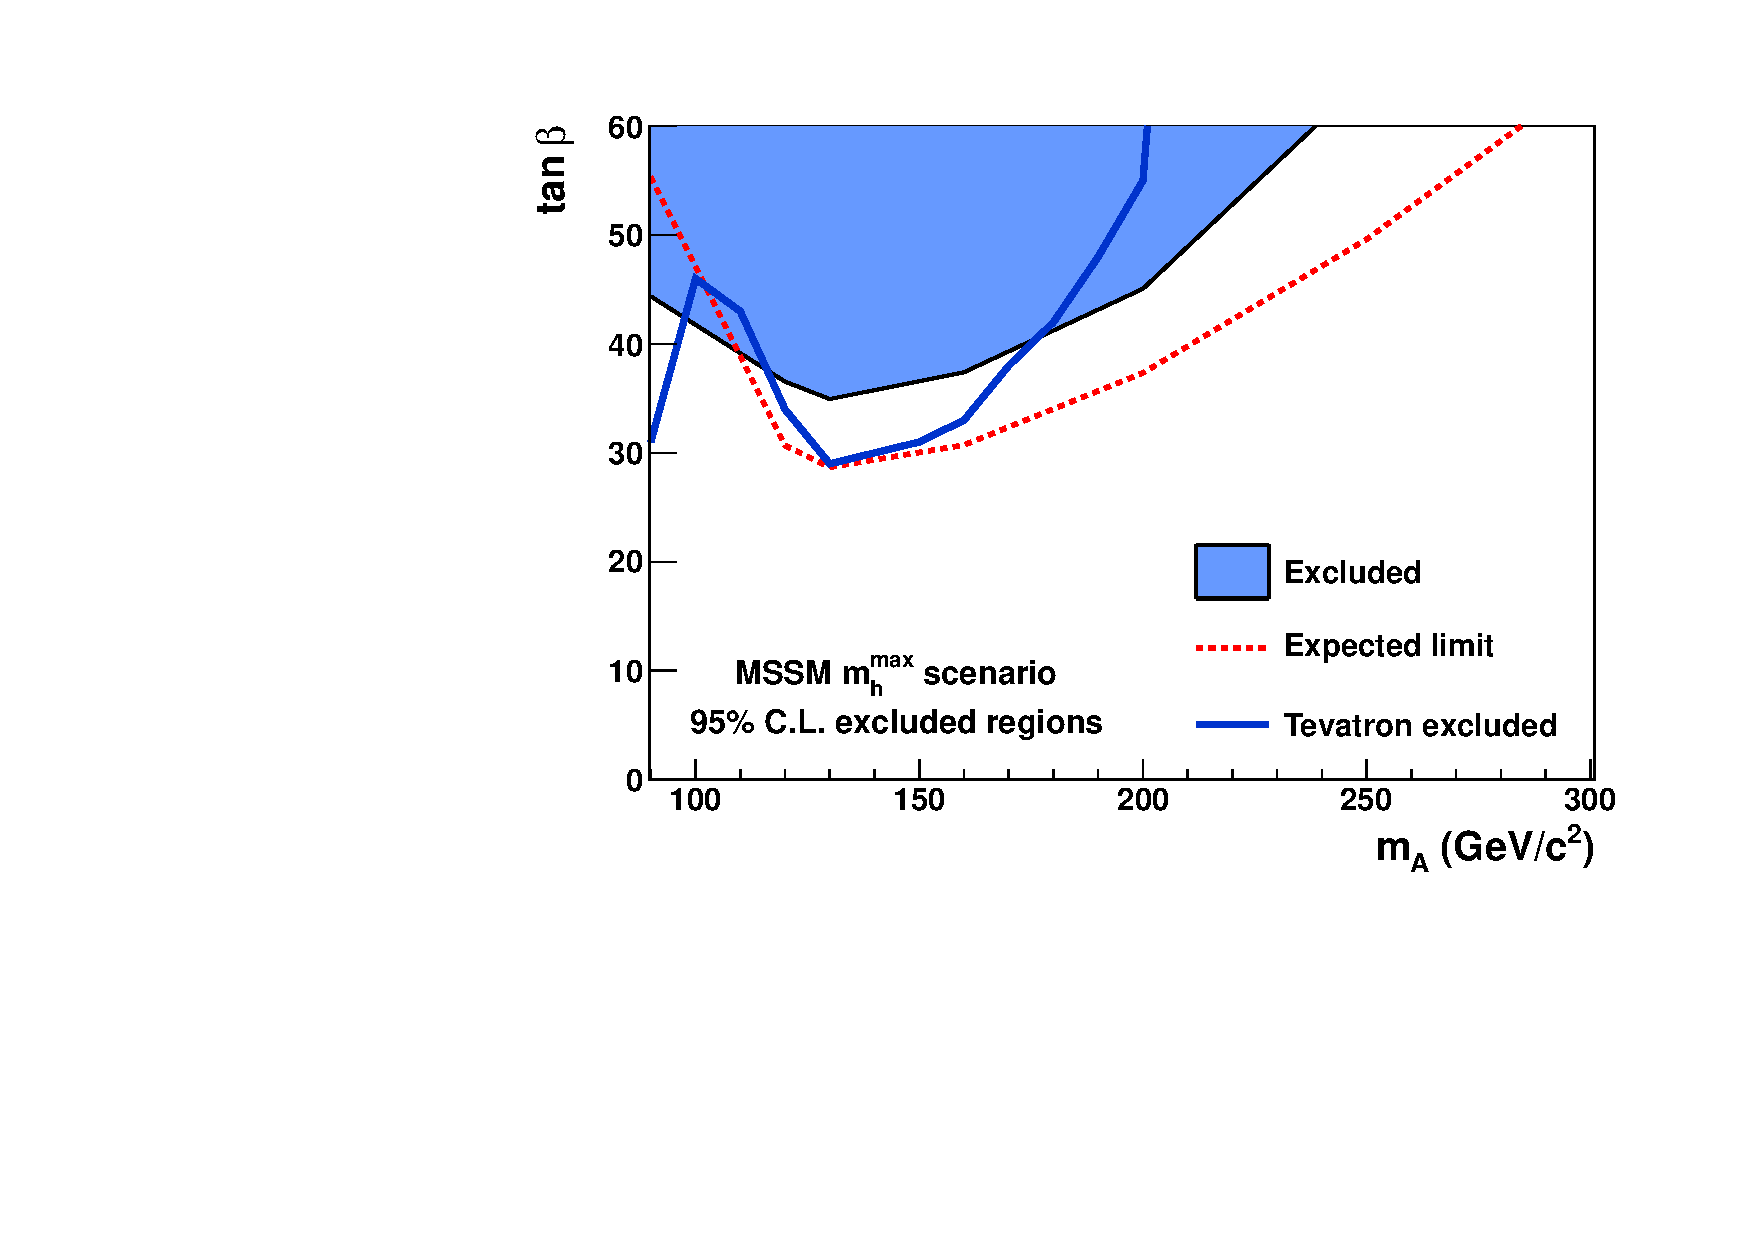
\includegraphics[width=\textwidth]{tools/tan_beta.pdf}
  \label{fig:TanBetaLimit} 
  \caption[Excluded regions of MSSM $\tb-\ma$ parameter space]{Region of MSSM
  $\tb-\ma$ parameter space excluded by this analysis.}
\end{figure}


\ifx\master\undefined% AUTOCOMPILE
% Allows for individual chapters to be compiled.

% Usage:
% \ifx\master\undefined% AUTOCOMPILE
% Allows for individual chapters to be compiled.

% Usage:
% \ifx\master\undefined% AUTOCOMPILE
% Allows for individual chapters to be compiled.

% Usage:
% \ifx\master\undefined\input{../settings/autocompile}\fi
% (place at start and end of chapter file)

\ifx\noprelim\undefined
    % first time included
    % input preamble files
    \input{../settings/phdsetup}

    \begin{document}
    \def\noprelim{}
\else
    % already included once
    % input post files

    \singlespacing
    \bibliographystyle{../bibliography/expanded}
    \bibliography{../bibliography/references}

    \end{document}
\fi\fi
% (place at start and end of chapter file)

\ifx\noprelim\undefined
    % first time included
    % input preamble files
    % [ USER VARIABLES ]

\def\PHDTITLE {Extensions of the Theory of Computational Mechanics}
\def\PHDAUTHOR{Evan Klose Friis}
\def\PHDSCHOOL{University of California, Davis}

\def\PHDMONTH {June}
\def\PHDYEAR  {2011}
\def\PHDDEPT {Physics}

\def\BSSCHOOL {University of California at San Diego}
\def\BSYEAR   {2005}

\def\PHDCOMMITTEEA{Professor John Conway}
\def\PHDCOMMITTEEB{Professor Robin Erbacher}
\def\PHDCOMMITTEEC{Professor Mani Tripathi}

% [ GLOBAL SETUP ]

\documentclass[letterpaper,oneside,11pt]{report}

\usepackage{calc}
\usepackage{breakcites}
\usepackage[newcommands]{ragged2e}

\usepackage[pdftex]{graphicx}
\usepackage{epstopdf}

%\usepackage{tikz}
%\usetikzlibrary{positioning} % [right=of ...]
%\usetikzlibrary{fit} % [fit= ...]

%\pgfdeclarelayer{background layer}
%\pgfdeclarelayer{foreground layer}
%\pgfsetlayers{background layer,main,foreground layer}

%\newenvironment{wrap}{\noindent\begin{minipage}[t]{\linewidth}\vspace{-0.5\normalbaselineskip}\centering}{\vspace{0.5\normalbaselineskip}\end{minipage}}

%% [Venn diagram environment]
%\newenvironment{venn2}
%{\begin{tikzpicture} [every pin/.style={text=black, text opacity=1.0, pin distance=0.5cm, pin edge={black!60, semithick}},
%% define a new style 'venn'
%venn/.style={circle, draw=black!60, semithick, minimum size = 4cm}]
%
%% create circle and give it external (pin) label
%\node[venn] (X) at (-1,0) [pin={150:$H[X]$}] {};
%\node[venn] (Y) at (1,0) [pin={30:$H[Y]$}] {};
%
%% place labels of the atoms by hand
%\node at (-1.9,0) {$H[X|Y]$};
%\node at (1.9,0) {$H[Y|X]$};
%\node at (0,0) {$I[X;Y]$};}
%{\end{tikzpicture}}

%\newcommand{\wrapmath}[1]{\begin{wrap}\begin{tikzpicture}[every node/.style={inner ysep=0ex, inner xsep=0em}]\node[] {$\displaystyle\begin{aligned} #1\end{aligned}$};\end{tikzpicture}\end{wrap}}

\renewenvironment{abstract}{\chapter*{Abstract}}{}
\renewcommand{\bibname}{Bibliography}
\renewcommand{\contentsname}{Table of Contents}

\makeatletter
\renewcommand{\@biblabel}[1]{\textsc{#1}}
\makeatother

% [ FONT SETTINGS ]

\usepackage[tbtags, intlimits, namelimits]{amsmath}
\usepackage[adobe-utopia]{mathdesign}

\DeclareSymbolFont{pazomath}{OMS}{zplm}{m}{n}
\DeclareSymbolFontAlphabet{\mathcal}{pazomath}
\SetMathAlphabet\mathcal{bold}{OMS}{zplm}{b}{n}

\SetSymbolFont{largesymbols}{normal}{OMX}{zplm}{m}{n}
\SetSymbolFont{largesymbols}{bold}{OMX}{zplm}{m}{n}
\SetSymbolFont{symbols}{normal}{OMS}{zplm}{m}{n}
\SetSymbolFont{symbols}{bold}{OMS}{zplm}{b}{n}

\renewcommand{\sfdefault}{phv}
\renewcommand{\ttdefault}{fvm}

\widowpenalty 8000
\clubpenalty  8000

% [ PAGE LAYOUT ]
\usepackage{geometry}
\geometry{lmargin = 1.5in}
\geometry{rmargin = 1.0in}
\geometry{tmargin = 1.0in}
\geometry{bmargin = 1.0in}

% [ PDF SETTINGS ]

\usepackage[final]{hyperref}
\hypersetup{breaklinks  = true}
\hypersetup{colorlinks  = true}
\hypersetup{linktocpage = false}
\hypersetup{linkcolor   = blue}
\hypersetup{citecolor   = green}
\hypersetup{urlcolor    = black}
\hypersetup{plainpages  = false}
\hypersetup{pageanchor  = true}
\hypersetup{pdfauthor   = {\PHDAUTHOR}}
\hypersetup{pdftitle    = {\PHDTITLE}}
\hypersetup{pdfsubject  = {Dissertation, \PHDSCHOOL}}
\urlstyle{same}

% [ LETTER SPACING ]

\usepackage[final]{microtype}
\microtypesetup{protrusion=compatibility}
\microtypesetup{expansion=false}

\newcommand{\upper}[1]{\MakeUppercase{#1}}
\let\lsscshape\scshape

\ifcase\pdfoutput\else\microtypesetup{letterspace=15}
\renewcommand{\scshape}{\lsscshape\lsstyle}
\renewcommand{\upper}[1]{\textls[50]{\MakeUppercase{#1}}}\fi

% [ LINE SPACING ]

\usepackage[doublespacing]{setspace}
\renewcommand{\displayskipstretch}{0.0}

\setlength{\parskip   }{0em}
\setlength{\parindent }{2em}

% [ TABLE FORMATTING ]

\usepackage{booktabs}
\setlength{\heavyrulewidth}{1.5\arrayrulewidth}
\setlength{\lightrulewidth}{1.0\arrayrulewidth}
\setlength{\doublerulesep }{2.0\arrayrulewidth}

% [ SECTION FORMATTING ]

\usepackage[largestsep,nobottomtitles*]{titlesec}
\renewcommand{\bottomtitlespace}{0.75in}

\titleformat{\chapter}[display]{\bfseries\huge\singlespacing}{\filleft\textsc{\LARGE \chaptertitlename\ \thechapter}}{-0.2ex}{\titlerule[3pt]\vspace{0.2ex}}[]

\titleformat{\section}{\LARGE}{\S\thesection\hspace{0.5em}}{0ex}{}
\titleformat{\subsection}{\Large}{\S\thesubsection\hspace{0.5em}}{0ex}{}
\titleformat{\subsubsection}{\large}{\thesubsubsection\hspace{0.5em}}{0ex}{}

\titlespacing*{\chapter}{0em}{6ex}{4ex plus 2ex minus 0ex}
\titlespacing*{\section}{0em}{2ex plus 3ex minus 1ex}{0.5ex plus 0.5ex minus 0.5ex}
\titlespacing*{\subsection}{0ex}{2ex plus 3ex minus 1ex}{0ex}
\titlespacing*{\subsubsection}{0ex}{2ex plus 0ex minus 1ex}{0ex}

% [ HEADER SETTINGS ]

\usepackage{fancyhdr}

\setlength{\headheight}{\normalbaselineskip}
\setlength{\footskip  }{0.5in}
\setlength{\headsep   }{0.5in-\headheight}

\fancyheadoffset[R]{0.5in}
\renewcommand{\headrulewidth}{0pt}
\renewcommand{\footrulewidth}{0pt}

\newcommand{\pagebox}{\parbox[r][\headheight][t]{0.5in}{\hspace\fill\thepage}}

\newcommand{\prelimheaders}{\ifx\prelim\undefined\renewcommand{\thepage}{\textit{\roman{page}}}\fancypagestyle{plain}{\fancyhf{}\fancyfoot[L]{\makebox[\textwidth-0.5in]{\thepage}}}\pagestyle{plain}\def\prelim{}\fi}

\newcommand{\normalheaders}{\renewcommand{\thepage}{\arabic{page}}\fancypagestyle{plain}{\fancyhf{}\fancyhead[R]{\pagebox}}\pagestyle{plain}}

\normalheaders{}

% [ CUSTOM COMMANDS ]

\newcommand{\signaturebox}[1]{\multicolumn{1}{p{4in}}{\vspace{3ex}}\\\midrule #1\\}

%\input{../includes/cmechabbrev}

% [some math stuff - maybe stick in sep file]
\usepackage{amsthm}
\usepackage{amscd}
\theoremstyle{plain}    \newtheorem{Lem}{Lemma}
\theoremstyle{plain}    \newtheorem*{ProLem}{Proof}
\theoremstyle{plain} 	\newtheorem{Cor}{Corollary}
\theoremstyle{plain} 	\newtheorem*{ProCor}{Proof}
\theoremstyle{plain} 	\newtheorem{The}{Theorem}
\theoremstyle{plain} 	\newtheorem*{ProThe}{Proof}
\theoremstyle{plain} 	\newtheorem{Prop}{Proposition}
\theoremstyle{plain} 	\newtheorem*{ProProp}{Proof}
\theoremstyle{plain} 	\newtheorem*{Conj}{Conjecture}
\theoremstyle{plain}	\newtheorem*{Rem}{Remark}
\theoremstyle{plain}	\newtheorem*{Def}{Definition} 
\theoremstyle{plain}	\newtheorem*{Not}{Notation}

% [uniform figure scaling - maybe this is not a good idea]
\def\figscale{.7}
\def\lscale{1.0}

% [FIX ME! - red makes it easier to spot]
\newcommand{\FIX}[1]{\textbf{\textcolor{red}{#1}}}


    \begin{document}
    \def\noprelim{}
\else
    % already included once
    % input post files

    \singlespacing
    \bibliographystyle{../bibliography/expanded}
    \bibliography{../bibliography/references}

    \end{document}
\fi\fi
% (place at start and end of chapter file)

\ifx\noprelim\undefined
    % first time included
    % input preamble files
    % [ USER VARIABLES ]

\def\PHDTITLE {Extensions of the Theory of Computational Mechanics}
\def\PHDAUTHOR{Evan Klose Friis}
\def\PHDSCHOOL{University of California, Davis}

\def\PHDMONTH {June}
\def\PHDYEAR  {2011}
\def\PHDDEPT {Physics}

\def\BSSCHOOL {University of California at San Diego}
\def\BSYEAR   {2005}

\def\PHDCOMMITTEEA{Professor John Conway}
\def\PHDCOMMITTEEB{Professor Robin Erbacher}
\def\PHDCOMMITTEEC{Professor Mani Tripathi}

% [ GLOBAL SETUP ]

\documentclass[letterpaper,oneside,11pt]{report}

\usepackage{calc}
\usepackage{breakcites}
\usepackage[newcommands]{ragged2e}

\usepackage[pdftex]{graphicx}
\usepackage{epstopdf}

%\usepackage{tikz}
%\usetikzlibrary{positioning} % [right=of ...]
%\usetikzlibrary{fit} % [fit= ...]

%\pgfdeclarelayer{background layer}
%\pgfdeclarelayer{foreground layer}
%\pgfsetlayers{background layer,main,foreground layer}

%\newenvironment{wrap}{\noindent\begin{minipage}[t]{\linewidth}\vspace{-0.5\normalbaselineskip}\centering}{\vspace{0.5\normalbaselineskip}\end{minipage}}

%% [Venn diagram environment]
%\newenvironment{venn2}
%{\begin{tikzpicture} [every pin/.style={text=black, text opacity=1.0, pin distance=0.5cm, pin edge={black!60, semithick}},
%% define a new style 'venn'
%venn/.style={circle, draw=black!60, semithick, minimum size = 4cm}]
%
%% create circle and give it external (pin) label
%\node[venn] (X) at (-1,0) [pin={150:$H[X]$}] {};
%\node[venn] (Y) at (1,0) [pin={30:$H[Y]$}] {};
%
%% place labels of the atoms by hand
%\node at (-1.9,0) {$H[X|Y]$};
%\node at (1.9,0) {$H[Y|X]$};
%\node at (0,0) {$I[X;Y]$};}
%{\end{tikzpicture}}

%\newcommand{\wrapmath}[1]{\begin{wrap}\begin{tikzpicture}[every node/.style={inner ysep=0ex, inner xsep=0em}]\node[] {$\displaystyle\begin{aligned} #1\end{aligned}$};\end{tikzpicture}\end{wrap}}

\renewenvironment{abstract}{\chapter*{Abstract}}{}
\renewcommand{\bibname}{Bibliography}
\renewcommand{\contentsname}{Table of Contents}

\makeatletter
\renewcommand{\@biblabel}[1]{\textsc{#1}}
\makeatother

% [ FONT SETTINGS ]

\usepackage[tbtags, intlimits, namelimits]{amsmath}
\usepackage[adobe-utopia]{mathdesign}

\DeclareSymbolFont{pazomath}{OMS}{zplm}{m}{n}
\DeclareSymbolFontAlphabet{\mathcal}{pazomath}
\SetMathAlphabet\mathcal{bold}{OMS}{zplm}{b}{n}

\SetSymbolFont{largesymbols}{normal}{OMX}{zplm}{m}{n}
\SetSymbolFont{largesymbols}{bold}{OMX}{zplm}{m}{n}
\SetSymbolFont{symbols}{normal}{OMS}{zplm}{m}{n}
\SetSymbolFont{symbols}{bold}{OMS}{zplm}{b}{n}

\renewcommand{\sfdefault}{phv}
\renewcommand{\ttdefault}{fvm}

\widowpenalty 8000
\clubpenalty  8000

% [ PAGE LAYOUT ]
\usepackage{geometry}
\geometry{lmargin = 1.5in}
\geometry{rmargin = 1.0in}
\geometry{tmargin = 1.0in}
\geometry{bmargin = 1.0in}

% [ PDF SETTINGS ]

\usepackage[final]{hyperref}
\hypersetup{breaklinks  = true}
\hypersetup{colorlinks  = true}
\hypersetup{linktocpage = false}
\hypersetup{linkcolor   = blue}
\hypersetup{citecolor   = green}
\hypersetup{urlcolor    = black}
\hypersetup{plainpages  = false}
\hypersetup{pageanchor  = true}
\hypersetup{pdfauthor   = {\PHDAUTHOR}}
\hypersetup{pdftitle    = {\PHDTITLE}}
\hypersetup{pdfsubject  = {Dissertation, \PHDSCHOOL}}
\urlstyle{same}

% [ LETTER SPACING ]

\usepackage[final]{microtype}
\microtypesetup{protrusion=compatibility}
\microtypesetup{expansion=false}

\newcommand{\upper}[1]{\MakeUppercase{#1}}
\let\lsscshape\scshape

\ifcase\pdfoutput\else\microtypesetup{letterspace=15}
\renewcommand{\scshape}{\lsscshape\lsstyle}
\renewcommand{\upper}[1]{\textls[50]{\MakeUppercase{#1}}}\fi

% [ LINE SPACING ]

\usepackage[doublespacing]{setspace}
\renewcommand{\displayskipstretch}{0.0}

\setlength{\parskip   }{0em}
\setlength{\parindent }{2em}

% [ TABLE FORMATTING ]

\usepackage{booktabs}
\setlength{\heavyrulewidth}{1.5\arrayrulewidth}
\setlength{\lightrulewidth}{1.0\arrayrulewidth}
\setlength{\doublerulesep }{2.0\arrayrulewidth}

% [ SECTION FORMATTING ]

\usepackage[largestsep,nobottomtitles*]{titlesec}
\renewcommand{\bottomtitlespace}{0.75in}

\titleformat{\chapter}[display]{\bfseries\huge\singlespacing}{\filleft\textsc{\LARGE \chaptertitlename\ \thechapter}}{-0.2ex}{\titlerule[3pt]\vspace{0.2ex}}[]

\titleformat{\section}{\LARGE}{\S\thesection\hspace{0.5em}}{0ex}{}
\titleformat{\subsection}{\Large}{\S\thesubsection\hspace{0.5em}}{0ex}{}
\titleformat{\subsubsection}{\large}{\thesubsubsection\hspace{0.5em}}{0ex}{}

\titlespacing*{\chapter}{0em}{6ex}{4ex plus 2ex minus 0ex}
\titlespacing*{\section}{0em}{2ex plus 3ex minus 1ex}{0.5ex plus 0.5ex minus 0.5ex}
\titlespacing*{\subsection}{0ex}{2ex plus 3ex minus 1ex}{0ex}
\titlespacing*{\subsubsection}{0ex}{2ex plus 0ex minus 1ex}{0ex}

% [ HEADER SETTINGS ]

\usepackage{fancyhdr}

\setlength{\headheight}{\normalbaselineskip}
\setlength{\footskip  }{0.5in}
\setlength{\headsep   }{0.5in-\headheight}

\fancyheadoffset[R]{0.5in}
\renewcommand{\headrulewidth}{0pt}
\renewcommand{\footrulewidth}{0pt}

\newcommand{\pagebox}{\parbox[r][\headheight][t]{0.5in}{\hspace\fill\thepage}}

\newcommand{\prelimheaders}{\ifx\prelim\undefined\renewcommand{\thepage}{\textit{\roman{page}}}\fancypagestyle{plain}{\fancyhf{}\fancyfoot[L]{\makebox[\textwidth-0.5in]{\thepage}}}\pagestyle{plain}\def\prelim{}\fi}

\newcommand{\normalheaders}{\renewcommand{\thepage}{\arabic{page}}\fancypagestyle{plain}{\fancyhf{}\fancyhead[R]{\pagebox}}\pagestyle{plain}}

\normalheaders{}

% [ CUSTOM COMMANDS ]

\newcommand{\signaturebox}[1]{\multicolumn{1}{p{4in}}{\vspace{3ex}}\\\midrule #1\\}

%%%% macros fro standard references
%\eqref provided by amsmath
\newcommand{\figref}[1]{Fig.~\ref{#1}}
\newcommand{\tableref}[1]{Table~\ref{#1}}
\newcommand{\refcite}[1]{Ref.~\cite{#1}}

% Abbreviations from CMPPSS:

\newcommand{\eM}     {\mbox{$\epsilon$-machine}}
\newcommand{\eMs}    {\mbox{$\epsilon$-machines}}
\newcommand{\EM}     {\mbox{$\epsilon$-Machine}}
\newcommand{\EMs}    {\mbox{$\epsilon$-Machines}}
\newcommand{\eT}     {\mbox{$\epsilon$-transducer}}
\newcommand{\eTs}    {\mbox{$\epsilon$-transducers}}
\newcommand{\ET}     {\mbox{$\epsilon$-Transducer}}
\newcommand{\ETs}    {\mbox{$\epsilon$-Transducers}}

% Processes and sequences

\newcommand{\Process}{\mathcal{P}}

\newcommand{\ProbMach}{\Prob_{\mathrm{M}}}
\newcommand{\Lmax}   { {L_{\mathrm{max}}}}
\newcommand{\MeasAlphabet}	{\mathcal{A}}
% Original
%\newcommand{\MeasSymbol}   { {S} }
%\newcommand{\meassymbol}   { {s} }
% New symbol
\newcommand{\MeasSymbol}   { {X} }
\newcommand{\meassymbol}   { {x} }
\newcommand{\BiInfinity}	{ \overleftrightarrow {\MeasSymbol} }
\newcommand{\biinfinity}	{ \overleftrightarrow {\meassymbol} }
\newcommand{\Past}	{ \overleftarrow {\MeasSymbol} }
\newcommand{\past}	{ {\overleftarrow {\meassymbol}} }
\newcommand{\pastprime}	{ {\past}^{\prime}}
\newcommand{\Future}	{ \overrightarrow{\MeasSymbol} }
\newcommand{\future}	{ \overrightarrow{\meassymbol} }
\newcommand{\futureprime}	{ {\future}^{\prime}}
\newcommand{\PastPrime}	{ {\Past}^{\prime}}
\newcommand{\FuturePrime}	{ {\overrightarrow{\meassymbol}}^\prime }
\newcommand{\PastDblPrime}	{ {\overleftarrow{\meassymbol}}^{\prime\prime} }
\newcommand{\FutureDblPrime}	{ {\overrightarrow{\meassymbol}}^{\prime\prime} }
\newcommand{\pastL}	{ {\overleftarrow {\meassymbol}}{}^L }
\newcommand{\PastL}	{ {\overleftarrow {\MeasSymbol}}{}^L }
\newcommand{\PastLt}	{ {\overleftarrow {\MeasSymbol}}_t^L }
\newcommand{\PastLLessOne}	{ {\overleftarrow {\MeasSymbol}}^{L-1} }
\newcommand{\futureL}	{ {\overrightarrow{\meassymbol}}{}^L }
\newcommand{\FutureL}	{ {\overrightarrow{\MeasSymbol}}{}^L }
\newcommand{\FutureLt}	{ {\overrightarrow{\MeasSymbol}}_t^L }
\newcommand{\FutureLLessOne}	{ {\overrightarrow{\MeasSymbol}}^{L-1} }
\newcommand{\pastLprime}	{ {\overleftarrow {\meassymbol}}^{L^\prime} }
\newcommand{\futureLprime}	{ {\overrightarrow{\meassymbol}}^{L^\prime} }
\newcommand{\AllPasts}	{ { \overleftarrow {\rm {\bf \MeasSymbol}} } }
\newcommand{\AllFutures}	{ \overrightarrow {\rm {\bf \MeasSymbol}} }
\newcommand{\FutureSet}	{ \overrightarrow{\bf \MeasSymbol}}

% Causal states and epsilon-machines
\newcommand{\CausalState}	{ \mathcal{S} }
\newcommand{\CausalStatePrime}	{ {\CausalState}^{\prime}}
\newcommand{\causalstate}	{ \sigma }
\newcommand{\CausalStateSet}	{ \boldsymbol{\CausalState} }
\newcommand{\AlternateState}	{ \mathcal{R} }
\newcommand{\AlternateStatePrime}	{ {\cal R}^{\prime} }
\newcommand{\alternatestate}	{ \rho }
\newcommand{\alternatestateprime}	{ {\rho^{\prime}} }
\newcommand{\AlternateStateSet}	{ \boldsymbol{\AlternateState} }
\newcommand{\PrescientState}	{ \widehat{\AlternateState} }
\newcommand{\prescientstate}	{ \widehat{\alternatestate} }
\newcommand{\PrescientStateSet}	{ \boldsymbol{\PrescientState}}
\newcommand{\CausalEquivalence}	{ {\sim}_{\epsilon} }
\newcommand{\CausalEquivalenceNot}	{ {\not \sim}_{\epsilon}}

\newcommand{\NonCausalEquivalence}	{ {\sim}_{\eta} }
\newcommand{\NextObservable}	{ {\overrightarrow {\MeasSymbol}}^1 }
\newcommand{\LastObservable}	{ {\overleftarrow {\MeasSymbol}}^1 }
%\newcommand{\Prob}		{ {\rm P}}
\newcommand{\Prob}      {\Pr} % use standard command
\newcommand{\ProbAnd}	{ {,\;} }
\newcommand{\LLimit}	{ {L \rightarrow \infty}}
\newcommand{\Cmu}		{C_\mu}
\newcommand{\hmu}		{h_\mu}
\newcommand{\EE}		{{\bf E}}
\newcommand{\Measurable}{{\bf \mu}}

% Process Crypticity
\newcommand{\PC}		{\chi}
\newcommand{\FuturePC}		{\PC^+}
\newcommand{\PastPC}		{\PC^-}
% Causal Irreversibility
\newcommand{\CI}		{\Xi}
\newcommand{\ReverseMap}	{r}
\newcommand{\ForwardMap}	{f}

% Abbreviations from IB:
% None that aren't already in CMPPSS

% Abbreviations from Extensive Estimation:
\newcommand{\EstCausalState}	{\widehat{\CausalState}}
\newcommand{\estcausalstate}	{\widehat{\causalstate}}
\newcommand{\EstCausalStateSet}	{\boldsymbol{\EstCausalState}}
\newcommand{\EstCausalFunc}	{\widehat{\epsilon}}
\newcommand{\EstCmu}		{\widehat{\Cmu}}
\newcommand{\PastLOne}	{{\Past}^{L+1}}
\newcommand{\pastLOne}	{{\past}^{L+1}}

% Abbreviations from $\epsilon$-Transducers:
\newcommand{\InAlphabet}	{ \mathcal{A}}
\newcommand{\insymbol}		{ a}
\newcommand{\OutAlphabet}	{ \mathcal{B}}
\newcommand{\outsymbol}		{ b}
\newcommand{\InputSimple}	{ X}
\newcommand{\inputsimple}	{ x}
\newcommand{\BottleneckVar}	{\tilde{\InputSimple}}
\newcommand{\bottleneckvar}	{\tilde{\inputsimple}}
\newcommand{\InputSpace}	{ \mathbf{\InputSimple}}
\newcommand{\InputBi}	{ \overleftrightarrow {\InputSimple} }
\newcommand{\inputbi}	{ \overleftrightarrow {\inputsimple} }
\newcommand{\InputPast}	{ \overleftarrow {\InputSimple} }
\newcommand{\inputpast}	{ \overleftarrow {\inputsimple} }
\newcommand{\InputFuture}	{ \overrightarrow {\InputSimple} }
\newcommand{\inputfuture}	{ \overrightarrow {\inputsimple} }
\newcommand{\NextInput}	{ {{\InputFuture}^{1}}}
\newcommand{\NextOutput}	{ {\OutputFuture}^{1}}
\newcommand{\OutputSimple}	{ Y}
\newcommand{\outputsimple}	{ y}
\newcommand{\OutputSpace}	{ \mathbf{\OutputSimple}}
\newcommand{\OutputBi}	{ \overleftrightarrow{\OutputSimple} }
\newcommand{\outputbi}	{ \overleftrightarrow{\outputsimple} }
\newcommand{\OutputPast}	{ \overleftarrow{\OutputSimple} }
\newcommand{\outputpast}	{ \overleftarrow{\outputsimple} }
\newcommand{\OutputFuture}	{ \overrightarrow{\OutputSimple} }
\newcommand{\outputfuture}	{ \overrightarrow{\outputsimple} }
\newcommand{\OutputL}	{ {\OutputFuture}^L}
\newcommand{\outputL}	{ {\outputfuture}^L}
\newcommand{\InputLLessOne}	{ {\InputFuture}^{L-1}}
\newcommand{\inputLlessone}	{ {\inputufutre}^{L-1}}
\newcommand{\OutputPastLLessOne}	{{\OutputPast}^{L-1}_{-1}}
\newcommand{\outputpastLlessone}	{{\outputpast}^{L-1}}
\newcommand{\OutputPastLessOne}	{{\OutputPast}_{-1}}
\newcommand{\outputpastlessone}	{{\outputpast}_{-1}}
\newcommand{\OutputPastL}	{{\OutputPast}^{L}}
\newcommand{\OutputLPlusOne}	{ {\OutputFuture}^{L+1}}
\newcommand{\outputLplusone}	{ {\outputfutre}^{L+1}}
\newcommand{\InputPastL}	{{\InputPast}^{L}}
\newcommand{\inputpastL}	{{\inputpast}^{L}}
\newcommand{\JointPast}	{{(\InputPast,\OutputPast)}}
\newcommand{\jointpast}	{{(\inputpast,\outputpast)}}
\newcommand{\jointpastone}	{{(\inputpast_1,\outputpast_1)}}
\newcommand{\jointpasttwo}	{{(\inputpast_2,\outputpast_2)}}
\newcommand{\jointpastprime} {{({\inputpast}^{\prime},{\outputpast}^{\prime})}}
\newcommand{\NextJoint}	{{(\NextInput,\NextOutput)}}
\newcommand{\nextjoint}	{{(\insymbol,\outsymbol)}}
\newcommand{\AllInputPasts}	{ { \overleftarrow {\rm \InputSpace}}}
\newcommand{\AllOutputPasts}	{ {\overleftarrow {\rm \OutputSpace}}}
\newcommand{\DetCausalState}	{ {{\cal S}_D }}
\newcommand{\detcausalstate}	{ {{\sigma}_D} }
\newcommand{\DetCausalStateSet}	{ \boldsymbol{{\CausalState}_D}}
\newcommand{\DetCausalEquivalence}	{ {\sim}_{{\epsilon}_{D}}}
\newcommand{\PrescientEquivalence}	{ {\sim}_{\widehat{\eta}}}
\newcommand{\FeedbackCausalState}	{ \mathcal{F}}
\newcommand{\feedbackcausalstate}	{ \phi}
\newcommand{\FeedbackCausalStateSet}	{ \mathbf{\FeedbackCausalState}}
\newcommand{\JointCausalState}		{ \mathcal{J}}
\newcommand{\JointCausalStateSet}	{ \mathbf{\JointCausalState}}
\newcommand{\UtilityFunctional}	{ {\mathcal{L}}}
\newcommand{\NatureState}	{ {\Omega}}
\newcommand{\naturestate}	{ {\omega}}
\newcommand{\NatureStateSpace}	{ {\mathbf{\NatureState}}}
\newcommand{\AnAction}	{ {A}}
\newcommand{\anaction}	{ {a}}
\newcommand{\ActionSpace}	{ {\mathbf{\AnAction}}}

% Abbreviations from RURO:
\newcommand{\InfoGain}[2] { \mathcal{D} \left( {#1} || {#2} \right) }

% Abbreviations from Upper Bound:
\newcommand{\lcm}	{{\rm lcm}}
% Double-check that this isn't in the math set already!

% Abbreviations from Emergence in Space
\newcommand{\ProcessAlphabet}	{\MeasAlphabet}
\newcommand{\ProbEst}			{ {\widehat{\Prob}_N}}
\newcommand{\STRegion}			{ {\mathrm K}}
\newcommand{\STRegionVariable}		{ K}
\newcommand{\stregionvariable}		{ k}
\newcommand{\GlobalPast}		{ \overleftarrow{G}} 
\newcommand{\globalpast}		{ \overleftarrow{g}} 
\newcommand{\GlobalFuture}		{ \overrightarrow{G}}
\newcommand{\globalfuture}		{ \overrightarrow{g}}
\newcommand{\GlobalState}		{ \mathcal{G}}
\newcommand{\globalstate}		{ \gamma}
\newcommand{\GlobalStateSet}		{ {\mathbf \GlobalState}}
\newcommand{\LocalPast}			{ \overleftarrow{L}} 
\newcommand{\localpast}			{ \overleftarrow{l}}
\newcommand{\AllLocalPasts}		{ \mathbf{\LocalPast}}
\newcommand{\LocalPastRegion}		{ \overleftarrow{\mathrm L}}
\newcommand{\LocalFuture}		{ \overrightarrow{L}}
\newcommand{\localfuture}		{ \overrightarrow{l}}
\newcommand{\LocalFutureRegion}		{ \overrightarrow{\mathrm L}}
\newcommand{\LocalState}		{ \mathcal{L}}
\newcommand{\localstate}		{ \lambda}
\newcommand{\LocalStateSet}		{ {\mathbf \LocalState}}
\newcommand{\PatchPast}			{ \overleftarrow{P}}
\newcommand{\patchpast}			{ \overleftarrow{p}}
\newcommand{\PatchPastRegion}		{ \overleftarrow{\mathrm P}}
\newcommand{\PatchFuture}		{ \overrightarrow{P}}
\newcommand{\patchfuture}		{ \overrightarrow{p}}
\newcommand{\PatchFutureRegion}		{ \overrightarrow{\mathrm P}}
\newcommand{\PatchState}		{ \mathcal{P}}
\newcommand{\patchstate}		{ \pi}
\newcommand{\PatchStateSet}		{ {\mathbf \PatchState}}
\newcommand{\LocalStatesInPatch}	{\vec{\LocalState}}
\newcommand{\localstatesinpatch}	{\vec{\localstate}}
\newcommand{\PointInstantX}		{ {\mathbf x}}
% Galles's original LaTeX for the cond. indep. symbol follows:
\newcommand{\compos}{\mbox{$~\underline{~\parallel~}~$}}
\newcommand{\ncompos}{\not\hspace{-.15in}\compos}
\newcommand{\indep}			{ \rotatebox{90}{$\models$}}
\newcommand{\nindep}	{\not\hspace{-.05in}\indep}
\newcommand{\LocalEE}	{{\EE}^{loc}}
\newcommand{\EEDensity}	{\overline{\LocalEE}}
\newcommand{\LocalCmu}	{{\Cmu}^{loc}}
\newcommand{\CmuDensity}	{\overline{\LocalCmu}}

%%%%%%%%%%% added by sasa
\newcommand{\FinPast}[1]	{ \overleftarrow {\MeasSymbol} \stackrel{{#1}}{}}
\newcommand{\finpast}[1]  	{ \overleftarrow {\meassymbol}  \stackrel{{#1}}{}}
\newcommand{\FinFuture}[1]		{ \overrightarrow{\MeasSymbol} \stackrel{{#1}}{}}
\newcommand{\finfuture}[1]		{ \overrightarrow{\meassymbol} \stackrel{{#1}}{}}

\newcommand{\Partition}	{ \AlternateState }
\newcommand{\partitionstate}	{ \alternatestate }
\newcommand{\PartitionSet}	{ \AlternateStateSet }
\newcommand{\Fdet}   { F_{\rm det} }

\newcommand{\Dkl}[2] { D_{\rm KL} \left( {#1} || {#2} \right) }

\newcommand{\Period}	{p}

% To take into account time direction
\newcommand{\forward}{+}
\newcommand{\reverse}{-}
%\newcommand{\forwardreverse}{\:\!\diamond} % \pm
\newcommand{\forwardreverse}{\pm} % \pm
\newcommand{\FutureProcess}	{ {\Process}^{\forward} }
\newcommand{\PastProcess}	{ {\Process}^{\reverse} }
\newcommand{\FutureCausalState}	{ {\CausalState}^{\forward} }
\newcommand{\futurecausalstate}	{ \sigma^{\forward} }
\newcommand{\altfuturecausalstate}	{ \sigma^{\forward\prime} }
\newcommand{\PastCausalState}	{ {\CausalState}^{\reverse} }
\newcommand{\pastcausalstate}	{ \sigma^{\reverse} }
\newcommand{\BiCausalState}		{ {\CausalState}^{\forwardreverse} }
\newcommand{\bicausalstate}		{ {\sigma}^{\forwardreverse} }
\newcommand{\FutureCausalStateSet}	{ {\CausalStateSet}^{\forward} }
\newcommand{\PastCausalStateSet}	{ {\CausalStateSet}^{\reverse} }
\newcommand{\BiCausalStateSet}	{ {\CausalStateSet}^{\forwardreverse} }
\newcommand{\eMachine}	{ M }
\newcommand{\FutureEM}	{ {\eMachine}^{\forward} }
\newcommand{\PastEM}	{ {\eMachine}^{\reverse} }
\newcommand{\BiEM}		{ {\eMachine}^{\forwardreverse} }
\newcommand{\BiEquiv}	{ {\sim}^{\forwardreverse} }
\newcommand{\Futurehmu}	{ h_\mu^{\forward} }
\newcommand{\Pasthmu}	{ h_\mu^{\reverse} }
\newcommand{\FutureCmu}	{ C_\mu^{\forward} }
\newcommand{\PastCmu}	{ C_\mu^{\reverse} }
\newcommand{\BiCmu}		{ C_\mu^{\forwardreverse} }
\newcommand{\FutureEps}	{ \epsilon^{\forward} }
\newcommand{\PastEps}	{ \epsilon^{\reverse} }
\newcommand{\BiEps}	{ \epsilon^{\forwardreverse} }
\newcommand{\FutureSim}	{ \sim^{\forward} }
\newcommand{\PastSim}	{ \sim^{\reverse} }
% Used arrows for awhile, more or less confusing?
%\newcommand{\FutureCausalState}	{ \overrightarrow{\CausalState} }
%\newcommand{\PastCausalState}	{ \overleftarrow{\CausalState} }
%\newcommand{\eMachine}	{ M }
%\newcommand{\FutureEM}	{ \overrightarrow{\eMachine} }
%\newcommand{\PastEM}	{ \overleftarrow{\eMachine} }
%\newcommand{\FutureCmu}	{ \overrightarrow{\Cmu} }
%\newcommand{\PastCmu}	{ \overleftarrow{\Cmu} }

%% time-reversing and mixed state presentation operators
\newcommand{\TR}{\mathcal{T}}
\newcommand{\MSP}{\mathcal{U}}
\newcommand{\one}{\mathbf{1}}

%% (cje)
%% Provide a command \ifpm which is true when \pm 
%% is meant to be understood as "+ or -". This is
%% different from the usage in TBA.
\newif\ifpm 
\edef\tempa{\forwardreverse}
\edef\tempb{\pm}
\ifx\tempa\tempb
   \pmfalse
\else
   \pmtrue  
\fi





% [some math stuff - maybe stick in sep file]
\usepackage{amsthm}
\usepackage{amscd}
\theoremstyle{plain}    \newtheorem{Lem}{Lemma}
\theoremstyle{plain}    \newtheorem*{ProLem}{Proof}
\theoremstyle{plain} 	\newtheorem{Cor}{Corollary}
\theoremstyle{plain} 	\newtheorem*{ProCor}{Proof}
\theoremstyle{plain} 	\newtheorem{The}{Theorem}
\theoremstyle{plain} 	\newtheorem*{ProThe}{Proof}
\theoremstyle{plain} 	\newtheorem{Prop}{Proposition}
\theoremstyle{plain} 	\newtheorem*{ProProp}{Proof}
\theoremstyle{plain} 	\newtheorem*{Conj}{Conjecture}
\theoremstyle{plain}	\newtheorem*{Rem}{Remark}
\theoremstyle{plain}	\newtheorem*{Def}{Definition} 
\theoremstyle{plain}	\newtheorem*{Not}{Notation}

% [uniform figure scaling - maybe this is not a good idea]
\def\figscale{.7}
\def\lscale{1.0}

% [FIX ME! - red makes it easier to spot]
\newcommand{\FIX}[1]{\textbf{\textcolor{red}{#1}}}


    \begin{document}
    \def\noprelim{}
\else
    % already included once
    % input post files

    \singlespacing
    \bibliographystyle{../bibliography/expanded}
    \bibliography{../bibliography/references}

    \end{document}
\fi\fi
